\documentclass{whiteboard}
\begin{document}
\begin{frame}[plain,t]
\bbcover{Grafos}{Algoritmo de Kruskal}{Prof. Edson Alves}{Faculdade UnB Gama}

\end{frame}
\begin{frame}[plain,t]
\begin{tikzpicture}
\node[draw,opacity=0] at (0, 0) {x};
\node[draw,opacity=0] at (14, 8) {x};

	\node[anchor=west] (title) at (0.0, 7.0) { \Large \bbbold{Proponente} };

	\node[] (floyd) at (7.0, 4.0) { \includegraphics[scale=0.4]{figs/kruskal.jpeg} };

	\node[] (fname) at (7.0, 1.0) { \bbbold{Joseph Bernard Kruskal, Jr.} };

	\node[] (fdate) at (7.0, 0.5) { \bbtext{(1962)} };

\end{tikzpicture}
\end{frame}
\begin{frame}[plain,t]
\begin{tikzpicture}
\node[draw,opacity=0] at (0, 0) {x};
\node[draw,opacity=0] at (14, 8) {x};

	\node[anchor=west] (title) at (0.0, 7.0) { \Large \bbbold{Características do algoritmo de Kruskal} };
\end{tikzpicture}
\end{frame}
\begin{frame}[plain,t]
\begin{tikzpicture}
\node[draw,opacity=0] at (0, 0) {x};
\node[draw,opacity=0] at (14, 8) {x};

	\node[anchor=west] (title) at (0.0, 7.0) { \Large \bbbold{Características do algoritmo de Kruskal} };

	\node[anchor=west] (a) at (1.0, 6.0) { $\star$ \bbtext{O algoritmo de Kruskal encontra uma MST usando uma abordagem gulosa} };

\end{tikzpicture}
\end{frame}
\begin{frame}[plain,t]
\begin{tikzpicture}
\node[draw,opacity=0] at (0, 0) {x};
\node[draw,opacity=0] at (14, 8) {x};

	\node[anchor=west] (title) at (0.0, 7.0) { \Large \bbbold{Características do algoritmo de Kruskal} };

	\node[anchor=west] (a) at (1.0, 6.0) { $\star$ \bbtext{O algoritmo de Kruskal encontra uma MST usando uma abordagem gulosa} };


	\node[anchor=west] (b) at (1.0, 5.0) { $\star$ \bbtext{As arestas são ordenadas, ascendentemente, por peso} };

\end{tikzpicture}
\end{frame}
\begin{frame}[plain,t]
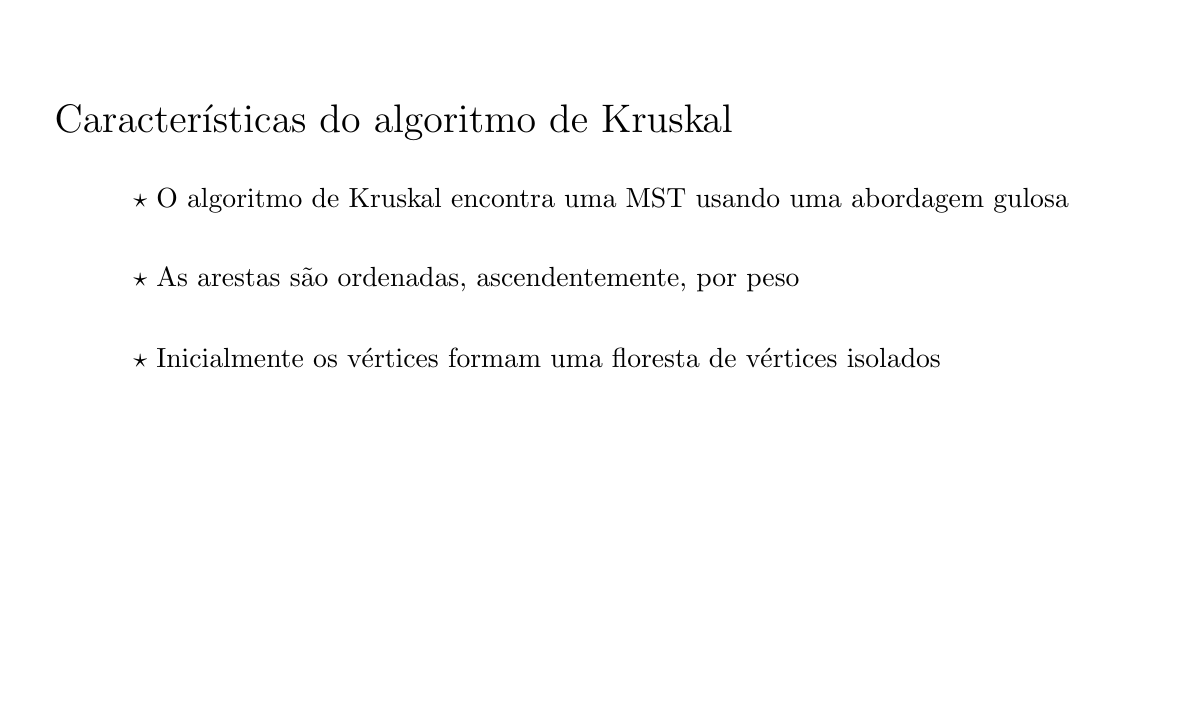
\begin{tikzpicture}
\node[draw,opacity=0] at (0, 0) {x};
\node[draw,opacity=0] at (14, 8) {x};

	\node[anchor=west] (title) at (0.0, 7.0) { \Large \bbbold{Características do algoritmo de Kruskal} };

	\node[anchor=west] (a) at (1.0, 6.0) { $\star$ \bbtext{O algoritmo de Kruskal encontra uma MST usando uma abordagem gulosa} };


	\node[anchor=west] (b) at (1.0, 5.0) { $\star$ \bbtext{As arestas são ordenadas, ascendentemente, por peso} };


	\node[anchor=west] (c) at (1.0, 4.0) { $\star$ \bbtext{Inicialmente os vértices formam uma floresta de vértices isolados} };

\end{tikzpicture}
\end{frame}
\begin{frame}[plain,t]
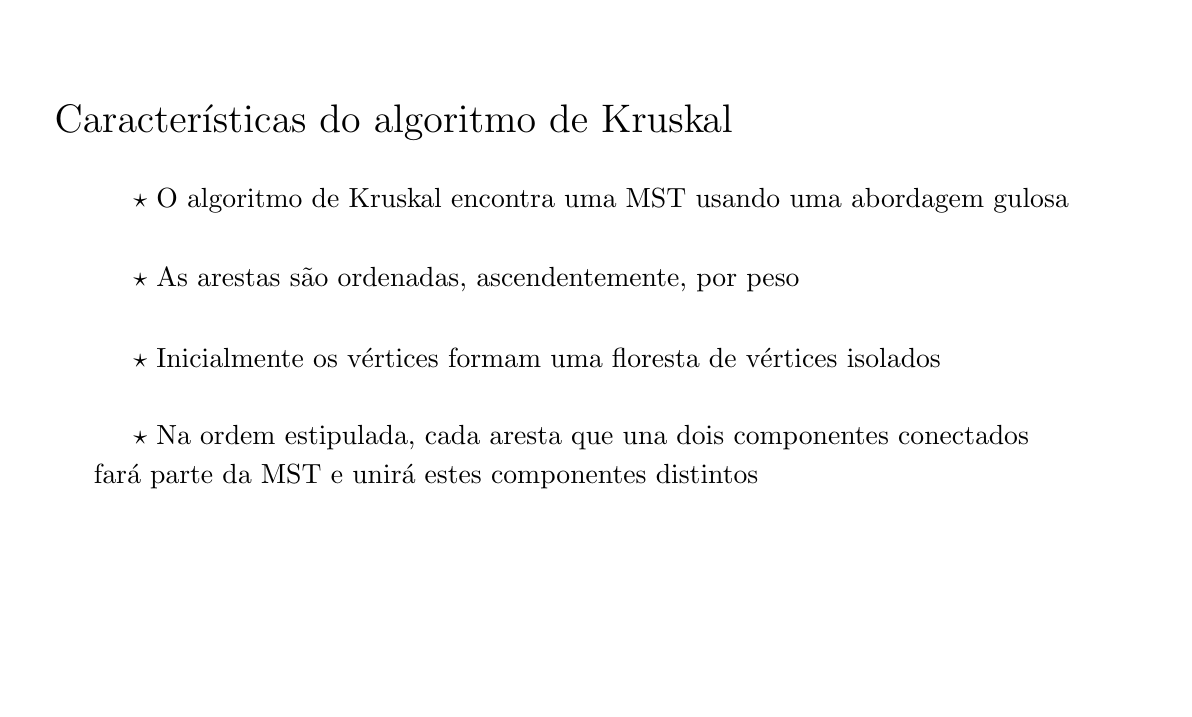
\begin{tikzpicture}
\node[draw,opacity=0] at (0, 0) {x};
\node[draw,opacity=0] at (14, 8) {x};

	\node[anchor=west] (title) at (0.0, 7.0) { \Large \bbbold{Características do algoritmo de Kruskal} };

	\node[anchor=west] (a) at (1.0, 6.0) { $\star$ \bbtext{O algoritmo de Kruskal encontra uma MST usando uma abordagem gulosa} };


	\node[anchor=west] (b) at (1.0, 5.0) { $\star$ \bbtext{As arestas são ordenadas, ascendentemente, por peso} };


	\node[anchor=west] (c) at (1.0, 4.0) { $\star$ \bbtext{Inicialmente os vértices formam uma floresta de vértices isolados} };


	\node[anchor=west] (d) at (1.0, 3.0) { $\star$ \bbtext{Na ordem estipulada, cada aresta que una dois componentes conectados} };

	\node[anchor=west] (d1) at (0.5, 2.5) { \bbtext{fará parte da MST e unirá estes componentes distintos} };


\end{tikzpicture}
\end{frame}
\begin{frame}[plain,t]
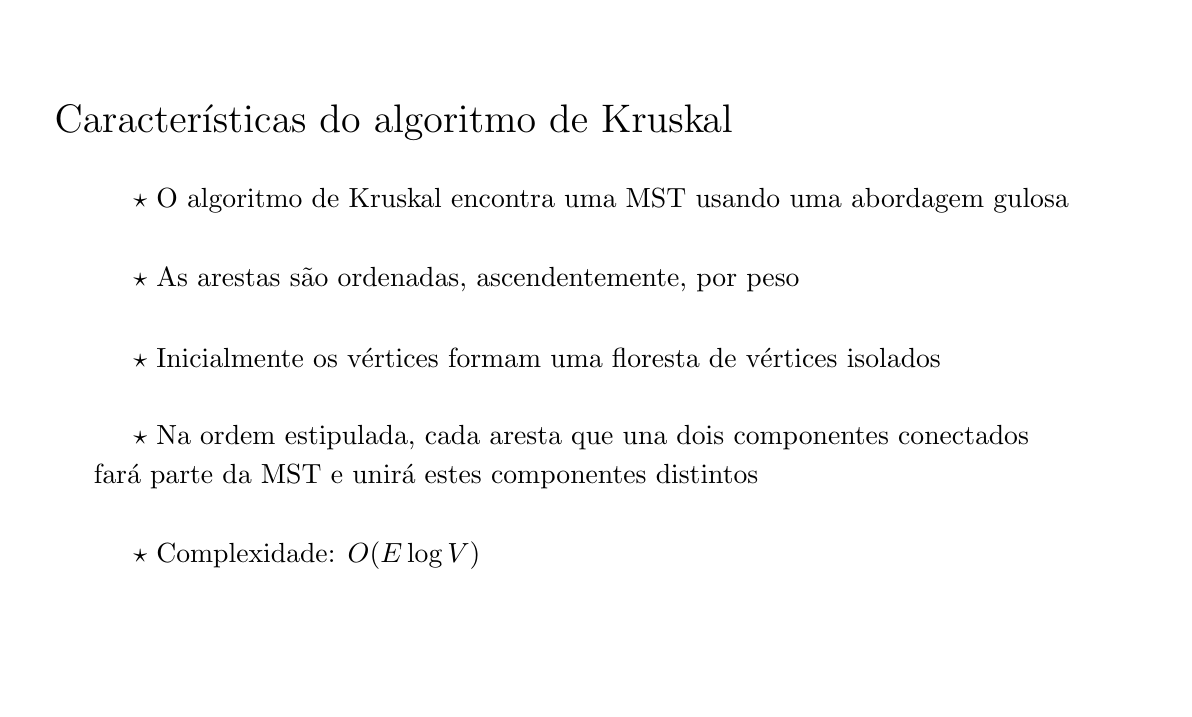
\begin{tikzpicture}
\node[draw,opacity=0] at (0, 0) {x};
\node[draw,opacity=0] at (14, 8) {x};

	\node[anchor=west] (title) at (0.0, 7.0) { \Large \bbbold{Características do algoritmo de Kruskal} };

	\node[anchor=west] (a) at (1.0, 6.0) { $\star$ \bbtext{O algoritmo de Kruskal encontra uma MST usando uma abordagem gulosa} };


	\node[anchor=west] (b) at (1.0, 5.0) { $\star$ \bbtext{As arestas são ordenadas, ascendentemente, por peso} };


	\node[anchor=west] (c) at (1.0, 4.0) { $\star$ \bbtext{Inicialmente os vértices formam uma floresta de vértices isolados} };


	\node[anchor=west] (d) at (1.0, 3.0) { $\star$ \bbtext{Na ordem estipulada, cada aresta que una dois componentes conectados} };

	\node[anchor=west] (d1) at (0.5, 2.5) { \bbtext{fará parte da MST e unirá estes componentes distintos} };



	\node[anchor=west] (e) at (1.0, 1.5) { $\star$ \bbtext{\bbbold{Complexidade}: $O(E\log V)$ } };

\end{tikzpicture}
\end{frame}
\begin{frame}[plain,t]
\begin{tikzpicture}
\node[draw,opacity=0] at (0, 0) {x};
\node[draw,opacity=0] at (14, 8) {x};

	\node[anchor=west] (title) at (0.0, 7.0) { \Large \bbbold{Pseudocódigo} };

\end{tikzpicture}
\end{frame}
\begin{frame}[plain,t]
\begin{tikzpicture}
\node[draw,opacity=0] at (0, 0) {x};
\node[draw,opacity=0] at (14, 8) {x};

	\node[anchor=west] (title) at (0.0, 7.0) { \Large \bbbold{Pseudocódigo} };


	\node[anchor=west] (input) at (0.5, 6.0) { \bbemph{Entrada:} \bbtext{um grafo ponderado $G(V, E)$} };

	\node[anchor=west] (output) at (0.5, 5.5) { \bbemph{Saída:} \bbtext{uma MST de $G$} };

\end{tikzpicture}
\end{frame}
\begin{frame}[plain,t]
\begin{tikzpicture}
\node[draw,opacity=0] at (0, 0) {x};
\node[draw,opacity=0] at (14, 8) {x};

	\node[anchor=west] (title) at (0.0, 7.0) { \Large \bbbold{Pseudocódigo} };


	\node[anchor=west] (input) at (0.5, 6.0) { \bbemph{Entrada:} \bbtext{um grafo ponderado $G(V, E)$} };

	\node[anchor=west] (output) at (0.5, 5.5) { \bbemph{Saída:} \bbtext{uma MST de $G$} };


	\node[anchor=west] (step1) at (1.0, 4.5) { $1.$ \bbtext{Faça $M = \emptyset$ e seja $F(V, \emptyset)$ uma floresta de vértices isolados} };

\end{tikzpicture}
\end{frame}
\begin{frame}[plain,t]
\begin{tikzpicture}
\node[draw,opacity=0] at (0, 0) {x};
\node[draw,opacity=0] at (14, 8) {x};

	\node[anchor=west] (title) at (0.0, 7.0) { \Large \bbbold{Pseudocódigo} };


	\node[anchor=west] (input) at (0.5, 6.0) { \bbemph{Entrada:} \bbtext{um grafo ponderado $G(V, E)$} };

	\node[anchor=west] (output) at (0.5, 5.5) { \bbemph{Saída:} \bbtext{uma MST de $G$} };


	\node[anchor=west] (step1) at (1.0, 4.5) { $1.$ \bbtext{Faça $M = \emptyset$ e seja $F(V, \emptyset)$ uma floresta de vértices isolados} };


	\node[anchor=west] (step2) at (1.0, 3.5) { $2.$ \bbtext{Ordene $E$ ascendentemente, por peso} };

\end{tikzpicture}
\end{frame}
\begin{frame}[plain,t]
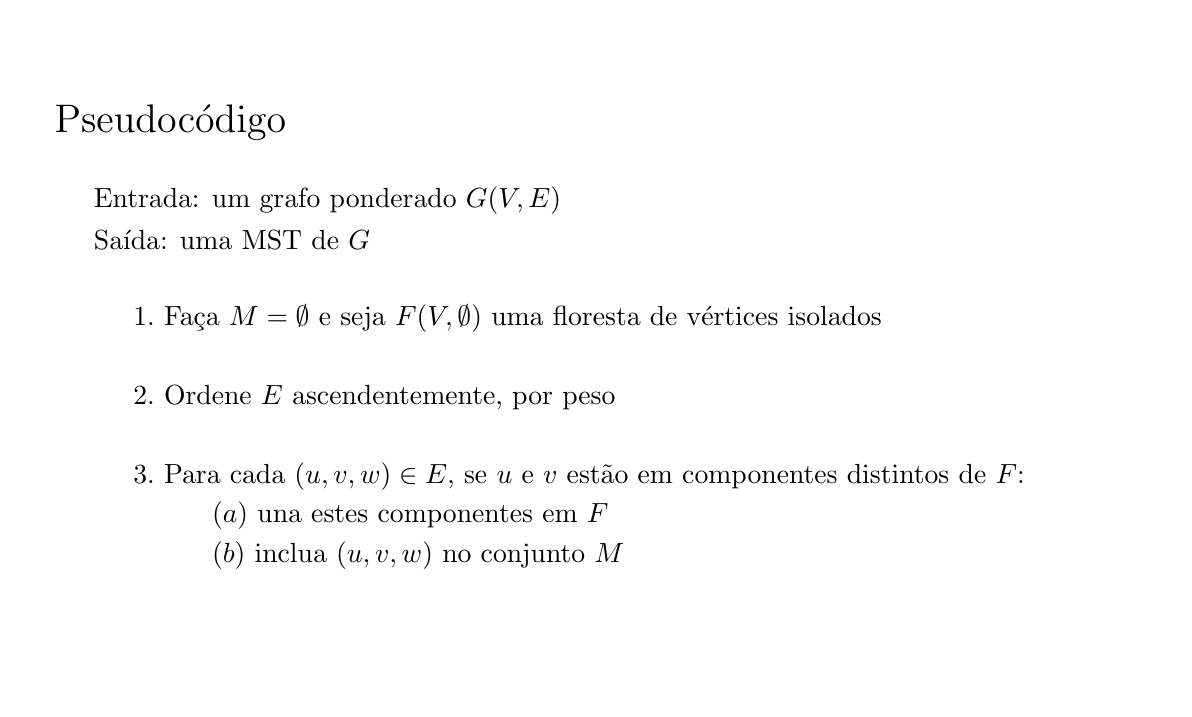
\begin{tikzpicture}
\node[draw,opacity=0] at (0, 0) {x};
\node[draw,opacity=0] at (14, 8) {x};

	\node[anchor=west] (title) at (0.0, 7.0) { \Large \bbbold{Pseudocódigo} };


	\node[anchor=west] (input) at (0.5, 6.0) { \bbemph{Entrada:} \bbtext{um grafo ponderado $G(V, E)$} };

	\node[anchor=west] (output) at (0.5, 5.5) { \bbemph{Saída:} \bbtext{uma MST de $G$} };


	\node[anchor=west] (step1) at (1.0, 4.5) { $1.$ \bbtext{Faça $M = \emptyset$ e seja $F(V, \emptyset)$ uma floresta de vértices isolados} };


	\node[anchor=west] (step2) at (1.0, 3.5) { $2.$ \bbtext{Ordene $E$ ascendentemente, por peso} };


	\node[anchor=west] (step3) at (1.0, 2.5) { $3.$ \bbtext{Para cada $(u, v, w)\in E$, se $u$ e $v$ estão em componentes distintos de $F$:} };

	\node[anchor=west] (step3a) at (2.0, 2.0) { $(a)$ \bbtext{una estes componentes em $F$} };

	\node[anchor=west] (step3b) at (2.0, 1.5) { $(b)$ \bbtext{inclua $(u, v, w)$ no conjunto $M$} };

\end{tikzpicture}
\end{frame}
\begin{frame}[plain,t]
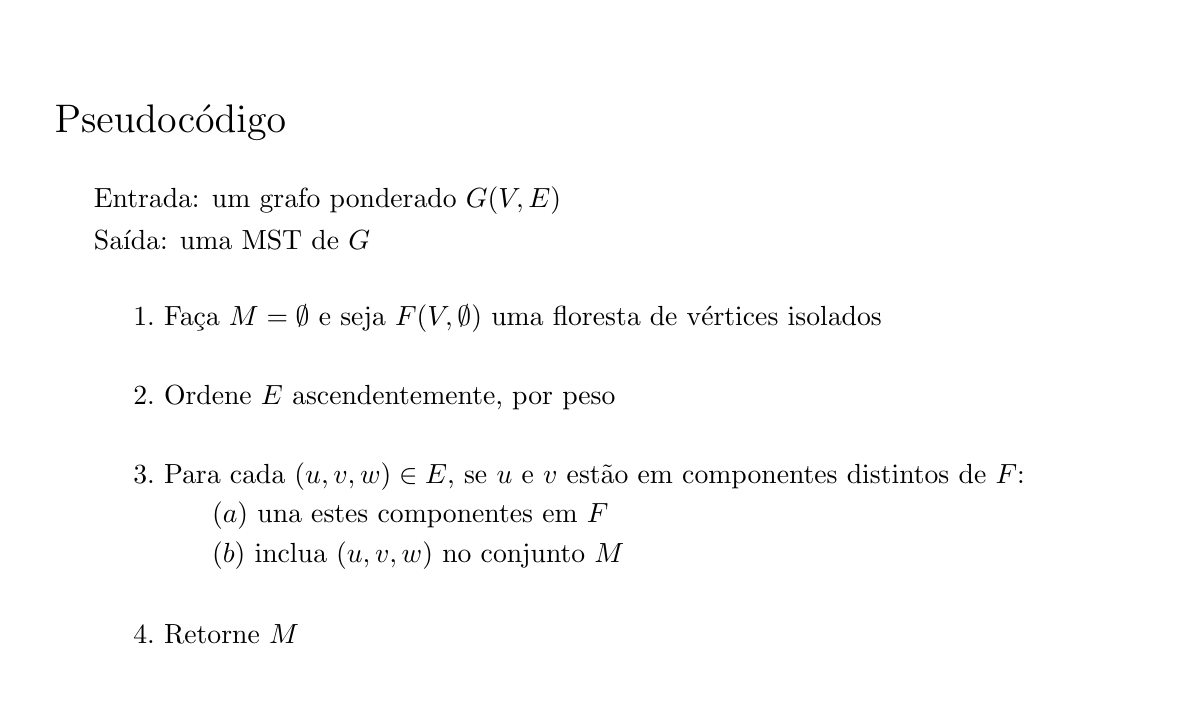
\begin{tikzpicture}
\node[draw,opacity=0] at (0, 0) {x};
\node[draw,opacity=0] at (14, 8) {x};

	\node[anchor=west] (title) at (0.0, 7.0) { \Large \bbbold{Pseudocódigo} };


	\node[anchor=west] (input) at (0.5, 6.0) { \bbemph{Entrada:} \bbtext{um grafo ponderado $G(V, E)$} };

	\node[anchor=west] (output) at (0.5, 5.5) { \bbemph{Saída:} \bbtext{uma MST de $G$} };


	\node[anchor=west] (step1) at (1.0, 4.5) { $1.$ \bbtext{Faça $M = \emptyset$ e seja $F(V, \emptyset)$ uma floresta de vértices isolados} };


	\node[anchor=west] (step2) at (1.0, 3.5) { $2.$ \bbtext{Ordene $E$ ascendentemente, por peso} };


	\node[anchor=west] (step3) at (1.0, 2.5) { $3.$ \bbtext{Para cada $(u, v, w)\in E$, se $u$ e $v$ estão em componentes distintos de $F$:} };

	\node[anchor=west] (step3a) at (2.0, 2.0) { $(a)$ \bbtext{una estes componentes em $F$} };

	\node[anchor=west] (step3b) at (2.0, 1.5) { $(b)$ \bbtext{inclua $(u, v, w)$ no conjunto $M$} };


	\node[anchor=west] (step4) at (1.0, 0.5) { $4.$ \bbtext{Retorne $M$} };

\end{tikzpicture}
\end{frame}
\begin{frame}[plain,t]
\begin{tikzpicture}
\node[draw,opacity=0] at (0, 0) {x};
\node[draw,opacity=0] at (14, 8) {x};

	\node[anchor=west] (x1) at (10.0, 6.0) { \bbtext{\tt 1 2 3} };

	\node[anchor=west] (x2) at (10.0, 5.5) { \bbtext{\tt 1 4 5} };

	\node[anchor=west] (x3) at (10.0, 5.0) { \bbtext{\tt 2 4 1} };

	\node[anchor=west] (x4) at (10.0, 4.5) { \bbtext{\tt 2 1 5} };

	\node[anchor=west] (x5) at (10.0, 4.0) { \bbtext{\tt 3 3 4} };

	\node[anchor=west] (x6) at (10.0, 3.5) { \bbtext{\tt 4 2 1} };

	\node[anchor=west] (x7) at (10.0, 3.0) { \bbtext{\tt 5 3 1} };

	\node[anchor=west] (x8) at (10.0, 2.5) { \bbtext{\tt 7 3 6} };

	\node[anchor=west] (x9) at (10.0, 2.0) { \bbtext{\tt 8 6 5} };

	\node[anchor=west] (E) at (10.4, 6.75) { \large $E$ };


	\node[very thick,draw,circle] (node1) at (6.0, 5.0) { \bbtext{1} };

	\node[very thick,draw,circle] (node2) at (4.0, 7.0) { \bbtext{2} };

	\node[very thick,draw,circle] (node3) at (2.0, 5.0) { \bbtext{3} };

	\node[very thick,draw,circle] (node4) at (6.0, 3.0) { \bbtext{4} };

	\node[very thick,draw,circle] (node5) at (4.0, 1.0) { \bbtext{5} };

	\node[very thick,draw,circle] (node6) at (2.0, 3.0) { \bbtext{6} };

\end{tikzpicture}
\end{frame}
\begin{frame}[plain,t]
\begin{tikzpicture}
\node[draw,opacity=0] at (0, 0) {x};
\node[draw,opacity=0] at (14, 8) {x};

	\node[anchor=west] (x1) at (10.0, 6.0) { \bbtext{\tt 1 2 3}\ \ \footnotesize{\textcolor{BBGreen}{\faCheck}} };

	\node[anchor=west] (x2) at (10.0, 5.5) { \bbtext{\tt 1 4 5} };

	\node[anchor=west] (x3) at (10.0, 5.0) { \bbtext{\tt 2 4 1} };

	\node[anchor=west] (x4) at (10.0, 4.5) { \bbtext{\tt 2 1 5} };

	\node[anchor=west] (x5) at (10.0, 4.0) { \bbtext{\tt 3 3 4} };

	\node[anchor=west] (x6) at (10.0, 3.5) { \bbtext{\tt 4 2 1} };

	\node[anchor=west] (x7) at (10.0, 3.0) { \bbtext{\tt 5 3 1} };

	\node[anchor=west] (x8) at (10.0, 2.5) { \bbtext{\tt 7 3 6} };

	\node[anchor=west] (x9) at (10.0, 2.0) { \bbtext{\tt 8 6 5} };

	\node[anchor=west] (E) at (10.4, 6.75) { \large $E$ };


	\node[very thick,draw,circle] (node1) at (6.0, 5.0) { \bbtext{1} };

	\node[very thick,draw,circle] (node2) at (4.0, 7.0) { \bbtext{2} };

	\node[very thick,draw,circle] (node3) at (2.0, 5.0) { \bbtext{3} };

	\node[very thick,draw,circle] (node4) at (6.0, 3.0) { \bbtext{4} };

	\node[very thick,draw,circle] (node5) at (4.0, 1.0) { \bbtext{5} };

	\node[very thick,draw,circle] (node6) at (2.0, 3.0) { \bbtext{6} };


	\draw[thick](node2) to node[above left] {\footnotesize \bbinfo{1}} (node3);


\end{tikzpicture}
\end{frame}
\begin{frame}[plain,t]
\begin{tikzpicture}
\node[draw,opacity=0] at (0, 0) {x};
\node[draw,opacity=0] at (14, 8) {x};

	\node[anchor=west] (x1) at (10.0, 6.0) { \bbtext{\tt 1 2 3}\ \ \footnotesize{\textcolor{BBGreen}{\faCheck}} };

	\node[anchor=west] (x2) at (10.0, 5.5) { \bbtext{\tt 1 4 5}\ \ \footnotesize{\textcolor{BBGreen}{\faCheck}} };

	\node[anchor=west] (x3) at (10.0, 5.0) { \bbtext{\tt 2 4 1} };

	\node[anchor=west] (x4) at (10.0, 4.5) { \bbtext{\tt 2 1 5} };

	\node[anchor=west] (x5) at (10.0, 4.0) { \bbtext{\tt 3 3 4} };

	\node[anchor=west] (x6) at (10.0, 3.5) { \bbtext{\tt 4 2 1} };

	\node[anchor=west] (x7) at (10.0, 3.0) { \bbtext{\tt 5 3 1} };

	\node[anchor=west] (x8) at (10.0, 2.5) { \bbtext{\tt 7 3 6} };

	\node[anchor=west] (x9) at (10.0, 2.0) { \bbtext{\tt 8 6 5} };

	\node[anchor=west] (E) at (10.4, 6.75) { \large $E$ };


	\node[very thick,draw,circle] (node1) at (6.0, 5.0) { \bbtext{1} };

	\node[very thick,draw,circle] (node2) at (4.0, 7.0) { \bbtext{2} };

	\node[very thick,draw,circle] (node3) at (2.0, 5.0) { \bbtext{3} };

	\node[very thick,draw,circle] (node4) at (6.0, 3.0) { \bbtext{4} };

	\node[very thick,draw,circle] (node5) at (4.0, 1.0) { \bbtext{5} };

	\node[very thick,draw,circle] (node6) at (2.0, 3.0) { \bbtext{6} };


	\draw[thick](node2) to node[above left] {\footnotesize \bbinfo{1}} (node3);



	\draw[thick](node4) to node[below right] {\footnotesize \bbinfo{1}} (node5);


\end{tikzpicture}
\end{frame}
\begin{frame}[plain,t]
\begin{tikzpicture}
\node[draw,opacity=0] at (0, 0) {x};
\node[draw,opacity=0] at (14, 8) {x};

	\node[anchor=west] (x1) at (10.0, 6.0) { \bbtext{\tt 1 2 3}\ \ \footnotesize{\textcolor{BBGreen}{\faCheck}} };

	\node[anchor=west] (x2) at (10.0, 5.5) { \bbtext{\tt 1 4 5}\ \ \footnotesize{\textcolor{BBGreen}{\faCheck}} };

	\node[anchor=west] (x3) at (10.0, 5.0) { \bbtext{\tt 2 4 1}\ \ \footnotesize{\textcolor{BBGreen}{\faCheck}} };

	\node[anchor=west] (x4) at (10.0, 4.5) { \bbtext{\tt 2 1 5} };

	\node[anchor=west] (x5) at (10.0, 4.0) { \bbtext{\tt 3 3 4} };

	\node[anchor=west] (x6) at (10.0, 3.5) { \bbtext{\tt 4 2 1} };

	\node[anchor=west] (x7) at (10.0, 3.0) { \bbtext{\tt 5 3 1} };

	\node[anchor=west] (x8) at (10.0, 2.5) { \bbtext{\tt 7 3 6} };

	\node[anchor=west] (x9) at (10.0, 2.0) { \bbtext{\tt 8 6 5} };

	\node[anchor=west] (E) at (10.4, 6.75) { \large $E$ };


	\node[very thick,draw,circle] (node1) at (6.0, 5.0) { \bbtext{1} };

	\node[very thick,draw,circle] (node2) at (4.0, 7.0) { \bbtext{2} };

	\node[very thick,draw,circle] (node3) at (2.0, 5.0) { \bbtext{3} };

	\node[very thick,draw,circle] (node4) at (6.0, 3.0) { \bbtext{4} };

	\node[very thick,draw,circle] (node5) at (4.0, 1.0) { \bbtext{5} };

	\node[very thick,draw,circle] (node6) at (2.0, 3.0) { \bbtext{6} };


	\draw[thick](node2) to node[above left] {\footnotesize \bbinfo{1}} (node3);



	\draw[thick](node4) to node[below right] {\footnotesize \bbinfo{1}} (node5);



	\draw[thick](node1) to node[right] {\footnotesize \bbinfo{2}} (node4);


\end{tikzpicture}
\end{frame}
\begin{frame}[plain,t]
\begin{tikzpicture}
\node[draw,opacity=0] at (0, 0) {x};
\node[draw,opacity=0] at (14, 8) {x};

	\node[anchor=west] (x1) at (10.0, 6.0) { \bbtext{\tt 1 2 3}\ \ \footnotesize{\textcolor{BBGreen}{\faCheck}} };

	\node[anchor=west] (x2) at (10.0, 5.5) { \bbtext{\tt 1 4 5}\ \ \footnotesize{\textcolor{BBGreen}{\faCheck}} };

	\node[anchor=west] (x3) at (10.0, 5.0) { \bbtext{\tt 2 4 1}\ \ \footnotesize{\textcolor{BBGreen}{\faCheck}} };

	\node[anchor=west] (x4) at (10.0, 4.5) { \bbtext{\tt 2 1 5}\ \ \footnotesize{\textcolor{BBRed}{\faClose}} };

	\node[anchor=west] (x5) at (10.0, 4.0) { \bbtext{\tt 3 3 4} };

	\node[anchor=west] (x6) at (10.0, 3.5) { \bbtext{\tt 4 2 1} };

	\node[anchor=west] (x7) at (10.0, 3.0) { \bbtext{\tt 5 3 1} };

	\node[anchor=west] (x8) at (10.0, 2.5) { \bbtext{\tt 7 3 6} };

	\node[anchor=west] (x9) at (10.0, 2.0) { \bbtext{\tt 8 6 5} };

	\node[anchor=west] (E) at (10.4, 6.75) { \large $E$ };


	\node[very thick,draw,circle] (node1) at (6.0, 5.0) { \bbtext{1} };

	\node[very thick,draw,circle] (node2) at (4.0, 7.0) { \bbtext{2} };

	\node[very thick,draw,circle] (node3) at (2.0, 5.0) { \bbtext{3} };

	\node[very thick,draw,circle] (node4) at (6.0, 3.0) { \bbtext{4} };

	\node[very thick,draw,circle] (node5) at (4.0, 1.0) { \bbtext{5} };

	\node[very thick,draw,circle] (node6) at (2.0, 3.0) { \bbtext{6} };


	\draw[thick](node2) to node[above left] {\footnotesize \bbinfo{1}} (node3);



	\draw[thick](node4) to node[below right] {\footnotesize \bbinfo{1}} (node5);



	\draw[thick](node1) to node[right] {\footnotesize \bbinfo{2}} (node4);




\end{tikzpicture}
\end{frame}
\begin{frame}[plain,t]
\begin{tikzpicture}
\node[draw,opacity=0] at (0, 0) {x};
\node[draw,opacity=0] at (14, 8) {x};

	\node[anchor=west] (x1) at (10.0, 6.0) { \bbtext{\tt 1 2 3}\ \ \footnotesize{\textcolor{BBGreen}{\faCheck}} };

	\node[anchor=west] (x2) at (10.0, 5.5) { \bbtext{\tt 1 4 5}\ \ \footnotesize{\textcolor{BBGreen}{\faCheck}} };

	\node[anchor=west] (x3) at (10.0, 5.0) { \bbtext{\tt 2 4 1}\ \ \footnotesize{\textcolor{BBGreen}{\faCheck}} };

	\node[anchor=west] (x4) at (10.0, 4.5) { \bbtext{\tt 2 1 5}\ \ \footnotesize{\textcolor{BBRed}{\faClose}} };

	\node[anchor=west] (x5) at (10.0, 4.0) { \bbtext{\tt 3 3 4}\ \ \footnotesize{\textcolor{BBGreen}{\faCheck}} };

	\node[anchor=west] (x6) at (10.0, 3.5) { \bbtext{\tt 4 2 1} };

	\node[anchor=west] (x7) at (10.0, 3.0) { \bbtext{\tt 5 3 1} };

	\node[anchor=west] (x8) at (10.0, 2.5) { \bbtext{\tt 7 3 6} };

	\node[anchor=west] (x9) at (10.0, 2.0) { \bbtext{\tt 8 6 5} };

	\node[anchor=west] (E) at (10.4, 6.75) { \large $E$ };


	\node[very thick,draw,circle] (node1) at (6.0, 5.0) { \bbtext{1} };

	\node[very thick,draw,circle] (node2) at (4.0, 7.0) { \bbtext{2} };

	\node[very thick,draw,circle] (node3) at (2.0, 5.0) { \bbtext{3} };

	\node[very thick,draw,circle] (node4) at (6.0, 3.0) { \bbtext{4} };

	\node[very thick,draw,circle] (node5) at (4.0, 1.0) { \bbtext{5} };

	\node[very thick,draw,circle] (node6) at (2.0, 3.0) { \bbtext{6} };


	\draw[thick](node2) to node[above left] {\footnotesize \bbinfo{1}} (node3);



	\draw[thick](node4) to node[below right] {\footnotesize \bbinfo{1}} (node5);



	\draw[thick](node1) to node[right] {\footnotesize \bbinfo{2}} (node4);





	\draw[thick](node3) to node[above] {\footnotesize \bbinfo{3}} (node4);


\end{tikzpicture}
\end{frame}
\begin{frame}[plain,t]
\begin{tikzpicture}
\node[draw,opacity=0] at (0, 0) {x};
\node[draw,opacity=0] at (14, 8) {x};

	\node[anchor=west] (x1) at (10.0, 6.0) { \bbtext{\tt 1 2 3}\ \ \footnotesize{\textcolor{BBGreen}{\faCheck}} };

	\node[anchor=west] (x2) at (10.0, 5.5) { \bbtext{\tt 1 4 5}\ \ \footnotesize{\textcolor{BBGreen}{\faCheck}} };

	\node[anchor=west] (x3) at (10.0, 5.0) { \bbtext{\tt 2 4 1}\ \ \footnotesize{\textcolor{BBGreen}{\faCheck}} };

	\node[anchor=west] (x4) at (10.0, 4.5) { \bbtext{\tt 2 1 5}\ \ \footnotesize{\textcolor{BBRed}{\faClose}} };

	\node[anchor=west] (x5) at (10.0, 4.0) { \bbtext{\tt 3 3 4}\ \ \footnotesize{\textcolor{BBGreen}{\faCheck}} };

	\node[anchor=west] (x6) at (10.0, 3.5) { \bbtext{\tt 4 2 1}\ \ \footnotesize{\textcolor{BBRed}{\faClose}} };

	\node[anchor=west] (x7) at (10.0, 3.0) { \bbtext{\tt 5 3 1} };

	\node[anchor=west] (x8) at (10.0, 2.5) { \bbtext{\tt 7 3 6} };

	\node[anchor=west] (x9) at (10.0, 2.0) { \bbtext{\tt 8 6 5} };

	\node[anchor=west] (E) at (10.4, 6.75) { \large $E$ };


	\node[very thick,draw,circle] (node1) at (6.0, 5.0) { \bbtext{1} };

	\node[very thick,draw,circle] (node2) at (4.0, 7.0) { \bbtext{2} };

	\node[very thick,draw,circle] (node3) at (2.0, 5.0) { \bbtext{3} };

	\node[very thick,draw,circle] (node4) at (6.0, 3.0) { \bbtext{4} };

	\node[very thick,draw,circle] (node5) at (4.0, 1.0) { \bbtext{5} };

	\node[very thick,draw,circle] (node6) at (2.0, 3.0) { \bbtext{6} };


	\draw[thick](node2) to node[above left] {\footnotesize \bbinfo{1}} (node3);



	\draw[thick](node4) to node[below right] {\footnotesize \bbinfo{1}} (node5);



	\draw[thick](node1) to node[right] {\footnotesize \bbinfo{2}} (node4);





	\draw[thick](node3) to node[above] {\footnotesize \bbinfo{3}} (node4);




\end{tikzpicture}
\end{frame}
\begin{frame}[plain,t]
\begin{tikzpicture}
\node[draw,opacity=0] at (0, 0) {x};
\node[draw,opacity=0] at (14, 8) {x};

	\node[anchor=west] (x1) at (10.0, 6.0) { \bbtext{\tt 1 2 3}\ \ \footnotesize{\textcolor{BBGreen}{\faCheck}} };

	\node[anchor=west] (x2) at (10.0, 5.5) { \bbtext{\tt 1 4 5}\ \ \footnotesize{\textcolor{BBGreen}{\faCheck}} };

	\node[anchor=west] (x3) at (10.0, 5.0) { \bbtext{\tt 2 4 1}\ \ \footnotesize{\textcolor{BBGreen}{\faCheck}} };

	\node[anchor=west] (x4) at (10.0, 4.5) { \bbtext{\tt 2 1 5}\ \ \footnotesize{\textcolor{BBRed}{\faClose}} };

	\node[anchor=west] (x5) at (10.0, 4.0) { \bbtext{\tt 3 3 4}\ \ \footnotesize{\textcolor{BBGreen}{\faCheck}} };

	\node[anchor=west] (x6) at (10.0, 3.5) { \bbtext{\tt 4 2 1}\ \ \footnotesize{\textcolor{BBRed}{\faClose}} };

	\node[anchor=west] (x7) at (10.0, 3.0) { \bbtext{\tt 5 3 1}\ \ \footnotesize{\textcolor{BBRed}{\faClose}} };

	\node[anchor=west] (x8) at (10.0, 2.5) { \bbtext{\tt 7 3 6} };

	\node[anchor=west] (x9) at (10.0, 2.0) { \bbtext{\tt 8 6 5} };

	\node[anchor=west] (E) at (10.4, 6.75) { \large $E$ };


	\node[very thick,draw,circle] (node1) at (6.0, 5.0) { \bbtext{1} };

	\node[very thick,draw,circle] (node2) at (4.0, 7.0) { \bbtext{2} };

	\node[very thick,draw,circle] (node3) at (2.0, 5.0) { \bbtext{3} };

	\node[very thick,draw,circle] (node4) at (6.0, 3.0) { \bbtext{4} };

	\node[very thick,draw,circle] (node5) at (4.0, 1.0) { \bbtext{5} };

	\node[very thick,draw,circle] (node6) at (2.0, 3.0) { \bbtext{6} };


	\draw[thick](node2) to node[above left] {\footnotesize \bbinfo{1}} (node3);



	\draw[thick](node4) to node[below right] {\footnotesize \bbinfo{1}} (node5);



	\draw[thick](node1) to node[right] {\footnotesize \bbinfo{2}} (node4);





	\draw[thick](node3) to node[above] {\footnotesize \bbinfo{3}} (node4);






\end{tikzpicture}
\end{frame}
\begin{frame}[plain,t]
\begin{tikzpicture}
\node[draw,opacity=0] at (0, 0) {x};
\node[draw,opacity=0] at (14, 8) {x};

	\node[anchor=west] (x1) at (10.0, 6.0) { \bbtext{\tt 1 2 3}\ \ \footnotesize{\textcolor{BBGreen}{\faCheck}} };

	\node[anchor=west] (x2) at (10.0, 5.5) { \bbtext{\tt 1 4 5}\ \ \footnotesize{\textcolor{BBGreen}{\faCheck}} };

	\node[anchor=west] (x3) at (10.0, 5.0) { \bbtext{\tt 2 4 1}\ \ \footnotesize{\textcolor{BBGreen}{\faCheck}} };

	\node[anchor=west] (x4) at (10.0, 4.5) { \bbtext{\tt 2 1 5}\ \ \footnotesize{\textcolor{BBRed}{\faClose}} };

	\node[anchor=west] (x5) at (10.0, 4.0) { \bbtext{\tt 3 3 4}\ \ \footnotesize{\textcolor{BBGreen}{\faCheck}} };

	\node[anchor=west] (x6) at (10.0, 3.5) { \bbtext{\tt 4 2 1}\ \ \footnotesize{\textcolor{BBRed}{\faClose}} };

	\node[anchor=west] (x7) at (10.0, 3.0) { \bbtext{\tt 5 3 1}\ \ \footnotesize{\textcolor{BBRed}{\faClose}} };

	\node[anchor=west] (x8) at (10.0, 2.5) { \bbtext{\tt 7 3 6}\ \ \footnotesize{\textcolor{BBGreen}{\faCheck}} };

	\node[anchor=west] (x9) at (10.0, 2.0) { \bbtext{\tt 8 6 5} };

	\node[anchor=west] (E) at (10.4, 6.75) { \large $E$ };


	\node[very thick,draw,circle] (node1) at (6.0, 5.0) { \bbtext{1} };

	\node[very thick,draw,circle] (node2) at (4.0, 7.0) { \bbtext{2} };

	\node[very thick,draw,circle] (node3) at (2.0, 5.0) { \bbtext{3} };

	\node[very thick,draw,circle] (node4) at (6.0, 3.0) { \bbtext{4} };

	\node[very thick,draw,circle] (node5) at (4.0, 1.0) { \bbtext{5} };

	\node[very thick,draw,circle] (node6) at (2.0, 3.0) { \bbtext{6} };


	\draw[thick](node2) to node[above left] {\footnotesize \bbinfo{1}} (node3);



	\draw[thick](node4) to node[below right] {\footnotesize \bbinfo{1}} (node5);



	\draw[thick](node1) to node[right] {\footnotesize \bbinfo{2}} (node4);





	\draw[thick](node3) to node[above] {\footnotesize \bbinfo{3}} (node4);







	\draw[thick](node3) to node[below left] {\footnotesize \bbinfo{7}} (node6);


\end{tikzpicture}
\end{frame}
\begin{frame}[plain,t]
\begin{tikzpicture}
\node[draw,opacity=0] at (0, 0) {x};
\node[draw,opacity=0] at (14, 8) {x};

	\node[anchor=west] (x1) at (10.0, 6.0) { \bbtext{\tt 1 2 3}\ \ \footnotesize{\textcolor{BBGreen}{\faCheck}} };

	\node[anchor=west] (x2) at (10.0, 5.5) { \bbtext{\tt 1 4 5}\ \ \footnotesize{\textcolor{BBGreen}{\faCheck}} };

	\node[anchor=west] (x3) at (10.0, 5.0) { \bbtext{\tt 2 4 1}\ \ \footnotesize{\textcolor{BBGreen}{\faCheck}} };

	\node[anchor=west] (x4) at (10.0, 4.5) { \bbtext{\tt 2 1 5}\ \ \footnotesize{\textcolor{BBRed}{\faClose}} };

	\node[anchor=west] (x5) at (10.0, 4.0) { \bbtext{\tt 3 3 4}\ \ \footnotesize{\textcolor{BBGreen}{\faCheck}} };

	\node[anchor=west] (x6) at (10.0, 3.5) { \bbtext{\tt 4 2 1}\ \ \footnotesize{\textcolor{BBRed}{\faClose}} };

	\node[anchor=west] (x7) at (10.0, 3.0) { \bbtext{\tt 5 3 1}\ \ \footnotesize{\textcolor{BBRed}{\faClose}} };

	\node[anchor=west] (x8) at (10.0, 2.5) { \bbtext{\tt 7 3 6}\ \ \footnotesize{\textcolor{BBGreen}{\faCheck}} };

	\node[anchor=west] (x9) at (10.0, 2.0) { \bbtext{\tt 8 6 5}\ \ \footnotesize{\textcolor{BBRed}{\faClose}} };

	\node[anchor=west] (E) at (10.4, 6.75) { \large $E$ };


	\node[very thick,draw,circle] (node1) at (6.0, 5.0) { \bbtext{1} };

	\node[very thick,draw,circle] (node2) at (4.0, 7.0) { \bbtext{2} };

	\node[very thick,draw,circle] (node3) at (2.0, 5.0) { \bbtext{3} };

	\node[very thick,draw,circle] (node4) at (6.0, 3.0) { \bbtext{4} };

	\node[very thick,draw,circle] (node5) at (4.0, 1.0) { \bbtext{5} };

	\node[very thick,draw,circle] (node6) at (2.0, 3.0) { \bbtext{6} };


	\draw[thick](node2) to node[above left] {\footnotesize \bbinfo{1}} (node3);



	\draw[thick](node4) to node[below right] {\footnotesize \bbinfo{1}} (node5);



	\draw[thick](node1) to node[right] {\footnotesize \bbinfo{2}} (node4);





	\draw[thick](node3) to node[above] {\footnotesize \bbinfo{3}} (node4);







	\draw[thick](node3) to node[below left] {\footnotesize \bbinfo{7}} (node6);




\end{tikzpicture}
\end{frame}
\begin{frame}[plain,t]
\begin{tikzpicture}
\node[draw,opacity=0] at (0, 0) {x};
\node[draw,opacity=0] at (14, 8) {x};

	\node[anchor=west] (title) at (0.0, 7.0) { \Large \bbbold{Identificação e união dos componentes conectados} };

\end{tikzpicture}
\end{frame}
\begin{frame}[plain,t]
\begin{tikzpicture}
\node[draw,opacity=0] at (0, 0) {x};
\node[draw,opacity=0] at (14, 8) {x};

	\node[anchor=west] (title) at (0.0, 7.0) { \Large \bbbold{Identificação e união dos componentes conectados} };


	\node[anchor=west] (a) at (1.0, 6.0) { $\star$ \bbtext{A complexidade do algoritmo de Kruskal depende da identificação e união} };

	\node[anchor=west] (a1) at (0.5, 5.5) { \bbtext{eficiente dos componentes conectados} };

\end{tikzpicture}
\end{frame}
\begin{frame}[plain,t]
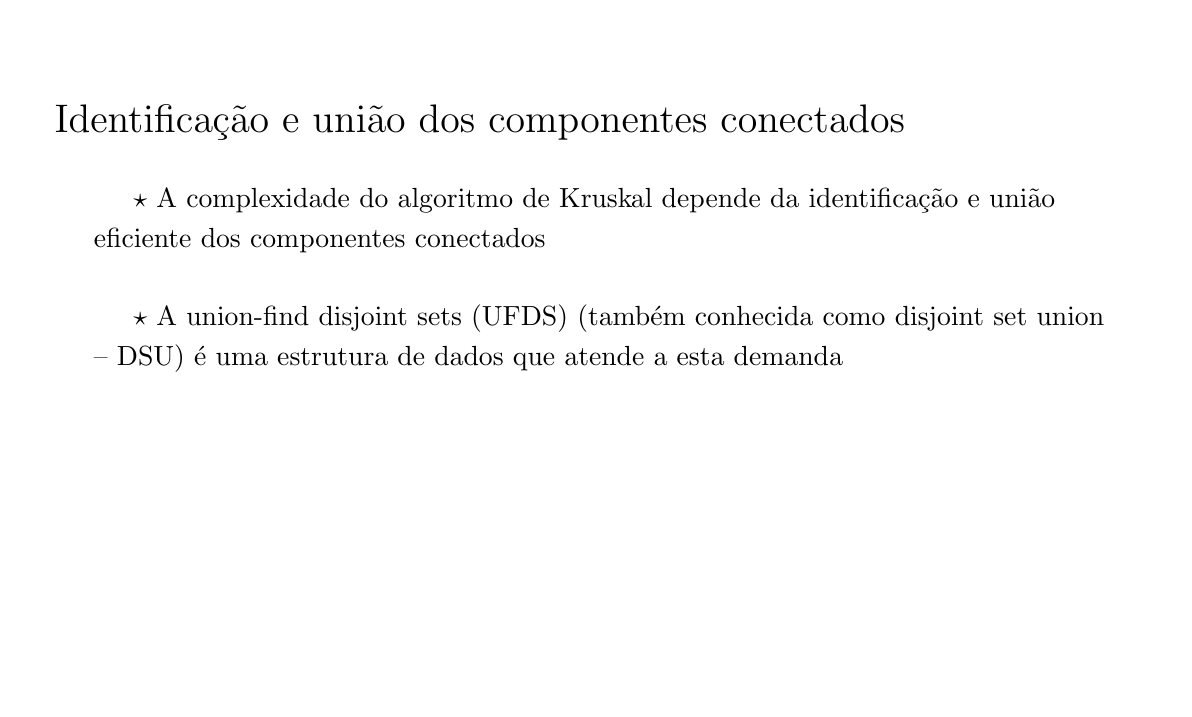
\begin{tikzpicture}
\node[draw,opacity=0] at (0, 0) {x};
\node[draw,opacity=0] at (14, 8) {x};

	\node[anchor=west] (title) at (0.0, 7.0) { \Large \bbbold{Identificação e união dos componentes conectados} };


	\node[anchor=west] (a) at (1.0, 6.0) { $\star$ \bbtext{A complexidade do algoritmo de Kruskal depende da identificação e união} };

	\node[anchor=west] (a1) at (0.5, 5.5) { \bbtext{eficiente dos componentes conectados} };


	\node[anchor=west] (b) at (1.0, 4.5) { $\star$ \bbtext{A \bbenglish{union-find disjoint sets} (UFDS) (também conhecida como \bbenglish{disjoint set union}} };

	\node[anchor=west] (b1) at (0.5, 4.0) { \bbtext{-- DSU) é uma estrutura de dados que atende a esta demanda} };


\end{tikzpicture}
\end{frame}
\begin{frame}[plain,t]
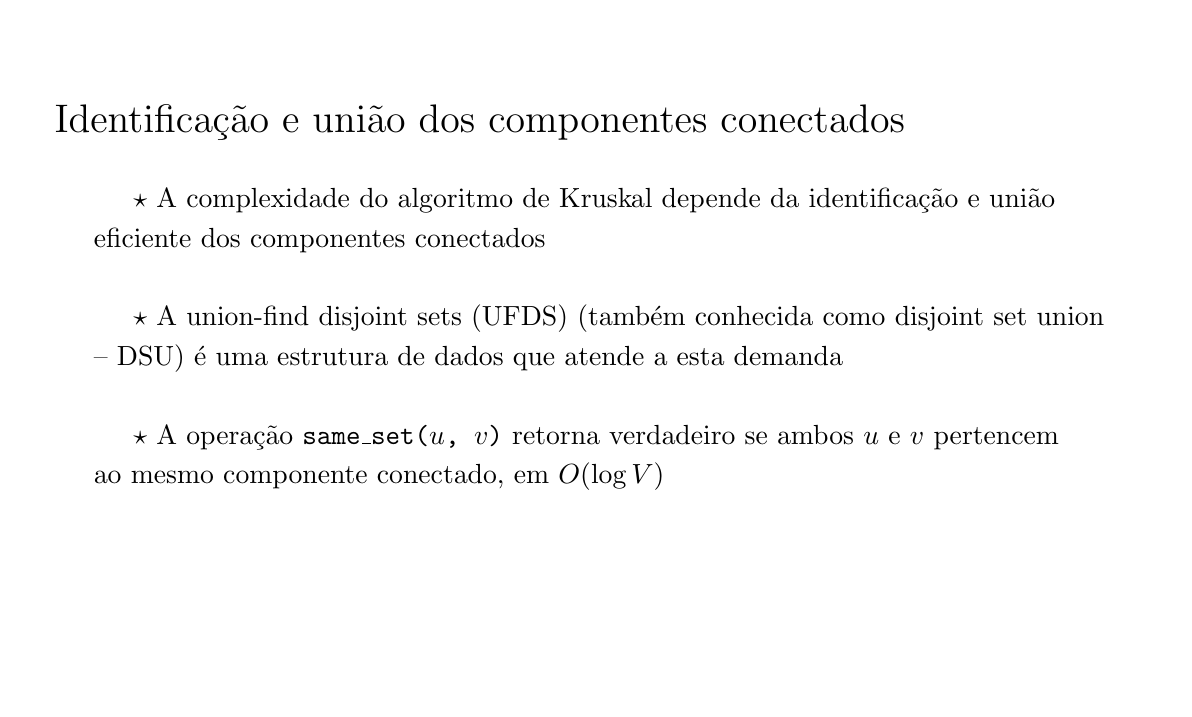
\begin{tikzpicture}
\node[draw,opacity=0] at (0, 0) {x};
\node[draw,opacity=0] at (14, 8) {x};

	\node[anchor=west] (title) at (0.0, 7.0) { \Large \bbbold{Identificação e união dos componentes conectados} };


	\node[anchor=west] (a) at (1.0, 6.0) { $\star$ \bbtext{A complexidade do algoritmo de Kruskal depende da identificação e união} };

	\node[anchor=west] (a1) at (0.5, 5.5) { \bbtext{eficiente dos componentes conectados} };


	\node[anchor=west] (b) at (1.0, 4.5) { $\star$ \bbtext{A \bbenglish{union-find disjoint sets} (UFDS) (também conhecida como \bbenglish{disjoint set union}} };

	\node[anchor=west] (b1) at (0.5, 4.0) { \bbtext{-- DSU) é uma estrutura de dados que atende a esta demanda} };



	\node[anchor=west] (c) at (1.0, 3.0) { $\star$ \bbtext{A operação \texttt{same\_set($u$, $v$)} retorna verdadeiro se ambos $u$ e $v$ pertencem} };

	\node[anchor=west] (c1) at (0.5, 2.5) { \bbtext{ao mesmo componente conectado, em $O(\log V)$} };

\end{tikzpicture}
\end{frame}
\begin{frame}[plain,t]
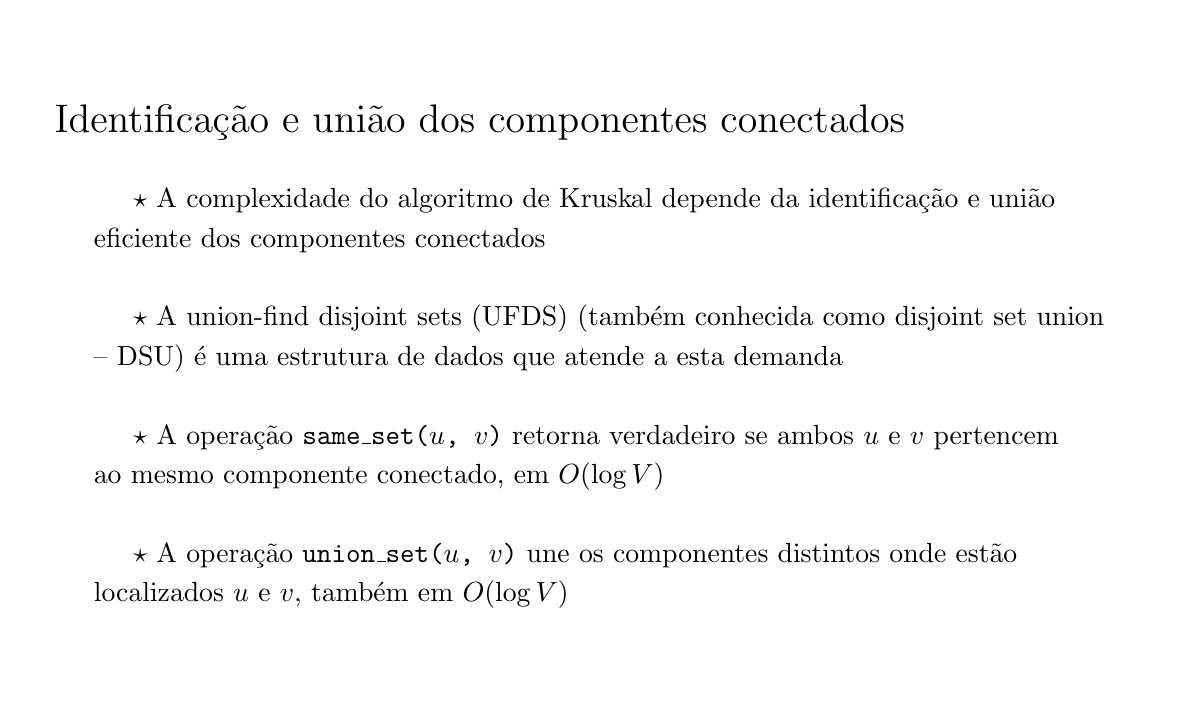
\begin{tikzpicture}
\node[draw,opacity=0] at (0, 0) {x};
\node[draw,opacity=0] at (14, 8) {x};

	\node[anchor=west] (title) at (0.0, 7.0) { \Large \bbbold{Identificação e união dos componentes conectados} };


	\node[anchor=west] (a) at (1.0, 6.0) { $\star$ \bbtext{A complexidade do algoritmo de Kruskal depende da identificação e união} };

	\node[anchor=west] (a1) at (0.5, 5.5) { \bbtext{eficiente dos componentes conectados} };


	\node[anchor=west] (b) at (1.0, 4.5) { $\star$ \bbtext{A \bbenglish{union-find disjoint sets} (UFDS) (também conhecida como \bbenglish{disjoint set union}} };

	\node[anchor=west] (b1) at (0.5, 4.0) { \bbtext{-- DSU) é uma estrutura de dados que atende a esta demanda} };



	\node[anchor=west] (c) at (1.0, 3.0) { $\star$ \bbtext{A operação \texttt{same\_set($u$, $v$)} retorna verdadeiro se ambos $u$ e $v$ pertencem} };

	\node[anchor=west] (c1) at (0.5, 2.5) { \bbtext{ao mesmo componente conectado, em $O(\log V)$} };


	\node[anchor=west] (d) at (1.0, 1.5) { $\star$ \bbtext{A operação \texttt{union\_set($u$, $v$)} une os componentes distintos onde estão} };

	\node[anchor=west] (d1) at (0.5, 1.0) { \bbtext{localizados $u$ e $v$, também em $O(\log V)$} };


\end{tikzpicture}
\end{frame}
\begin{frame}[plain,t]

\inputsnippet{cpp}{46}{63}{codes/kruskal.cpp}

\end{frame}
\begin{frame}[plain,t]
\begin{tikzpicture}
\node[draw,opacity=0] at (0, 0) {x};
\node[draw,opacity=0] at (14, 8) {x};

	\node[anchor=west] (title) at (0.0, 6.5) { \Large \bbbold{Aplicação: Floresta mínima geradora} };

\end{tikzpicture}
\end{frame}
\begin{frame}[plain,t]
\begin{tikzpicture}
\node[draw,opacity=0] at (0, 0) {x};
\node[draw,opacity=0] at (14, 8) {x};

	\node[anchor=west] (title) at (0.0, 6.5) { \Large \bbbold{Aplicação: Floresta mínima geradora} };


	\node[anchor=west] (a) at (1.0, 5.5) { $\star$ \bbtext{Uma floresta mínima geradora $F_k$ pode ser identificada por meio de uma} };

	\node[anchor=west] (a1) at (0.5, 5.0) { \bbtext{modificação simples no algoritmo de Kruskal} };

\end{tikzpicture}
\end{frame}
\begin{frame}[plain,t]
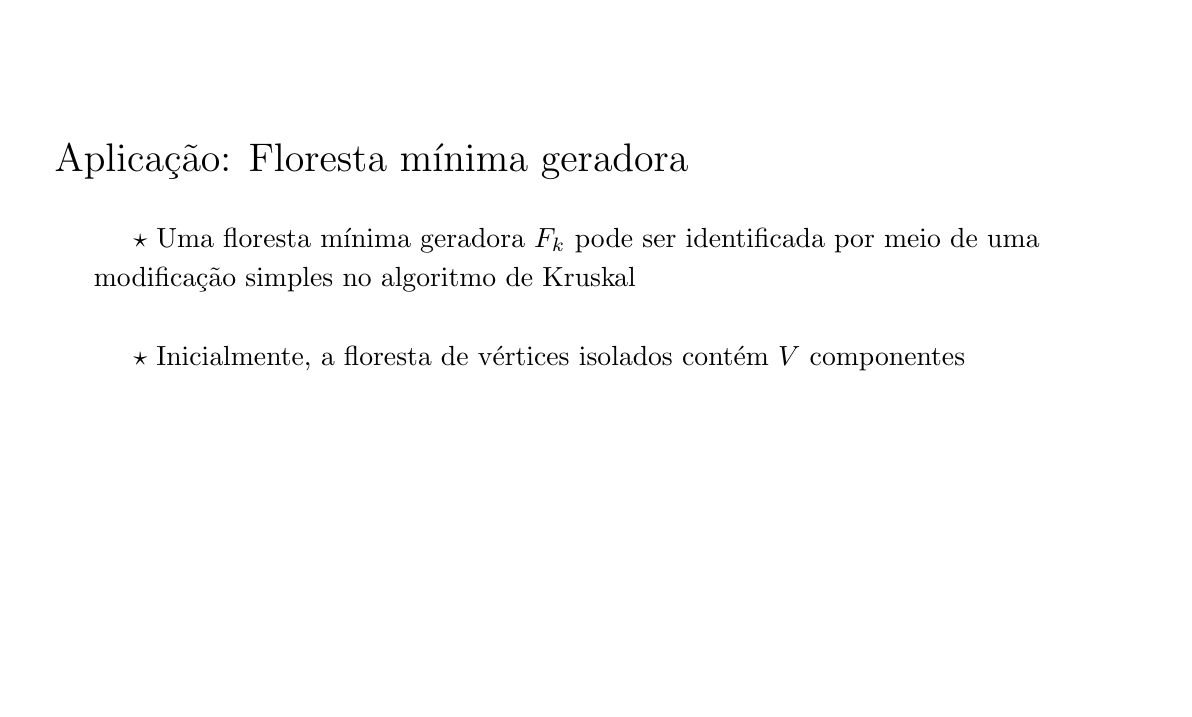
\begin{tikzpicture}
\node[draw,opacity=0] at (0, 0) {x};
\node[draw,opacity=0] at (14, 8) {x};

	\node[anchor=west] (title) at (0.0, 6.5) { \Large \bbbold{Aplicação: Floresta mínima geradora} };


	\node[anchor=west] (a) at (1.0, 5.5) { $\star$ \bbtext{Uma floresta mínima geradora $F_k$ pode ser identificada por meio de uma} };

	\node[anchor=west] (a1) at (0.5, 5.0) { \bbtext{modificação simples no algoritmo de Kruskal} };


	\node[anchor=west] (b) at (1.0, 4.0) { $\star$ \bbtext{Inicialmente, a floresta de vértices isolados contém $V$ componentes} };

\end{tikzpicture}
\end{frame}
\begin{frame}[plain,t]
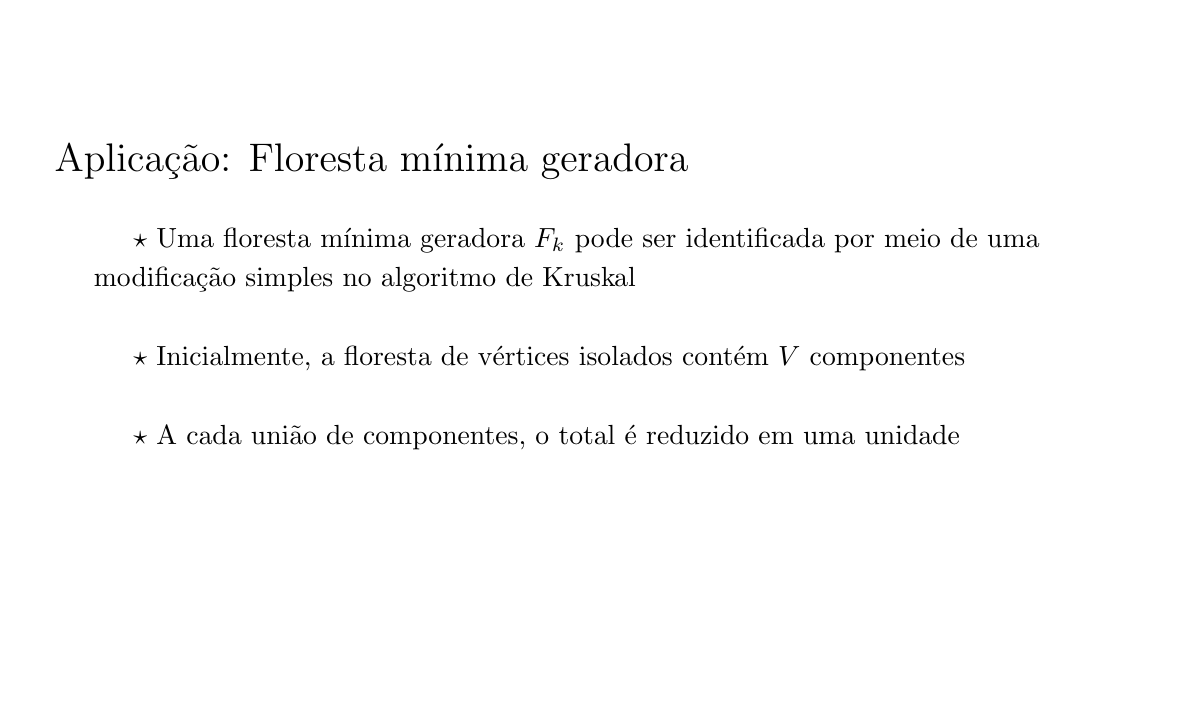
\begin{tikzpicture}
\node[draw,opacity=0] at (0, 0) {x};
\node[draw,opacity=0] at (14, 8) {x};

	\node[anchor=west] (title) at (0.0, 6.5) { \Large \bbbold{Aplicação: Floresta mínima geradora} };


	\node[anchor=west] (a) at (1.0, 5.5) { $\star$ \bbtext{Uma floresta mínima geradora $F_k$ pode ser identificada por meio de uma} };

	\node[anchor=west] (a1) at (0.5, 5.0) { \bbtext{modificação simples no algoritmo de Kruskal} };


	\node[anchor=west] (b) at (1.0, 4.0) { $\star$ \bbtext{Inicialmente, a floresta de vértices isolados contém $V$ componentes} };


	\node[anchor=west] (c) at (1.0, 3.0) { $\star$ \bbtext{A cada união de componentes, o total é reduzido em uma unidade} };

\end{tikzpicture}
\end{frame}
\begin{frame}[plain,t]
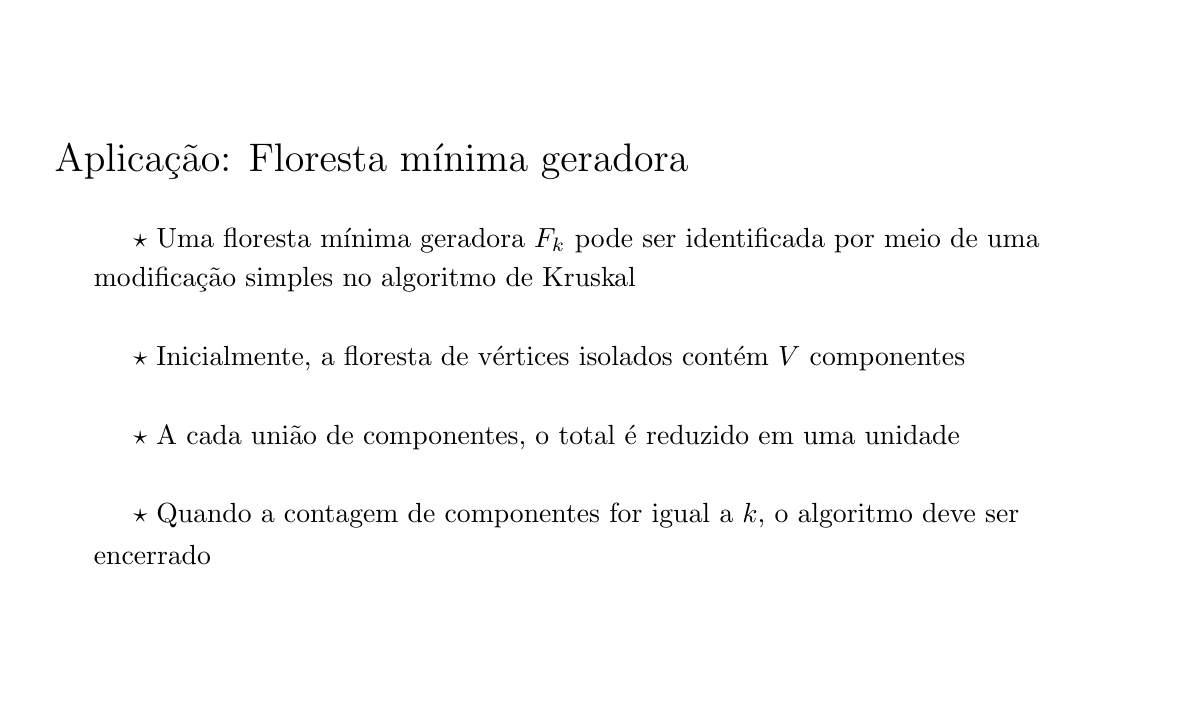
\begin{tikzpicture}
\node[draw,opacity=0] at (0, 0) {x};
\node[draw,opacity=0] at (14, 8) {x};

	\node[anchor=west] (title) at (0.0, 6.5) { \Large \bbbold{Aplicação: Floresta mínima geradora} };


	\node[anchor=west] (a) at (1.0, 5.5) { $\star$ \bbtext{Uma floresta mínima geradora $F_k$ pode ser identificada por meio de uma} };

	\node[anchor=west] (a1) at (0.5, 5.0) { \bbtext{modificação simples no algoritmo de Kruskal} };


	\node[anchor=west] (b) at (1.0, 4.0) { $\star$ \bbtext{Inicialmente, a floresta de vértices isolados contém $V$ componentes} };


	\node[anchor=west] (c) at (1.0, 3.0) { $\star$ \bbtext{A cada união de componentes, o total é reduzido em uma unidade} };


	\node[anchor=west] (d) at (1.0, 2.0) { $\star$ \bbtext{Quando a contagem de componentes for igual a $k$, o algoritmo deve ser } };

	\node[anchor=west] (d1) at (0.5, 1.5) { \bbtext{encerrado} };

\end{tikzpicture}
\end{frame}
\begin{frame}[plain,t]
\begin{tikzpicture}
\node[draw,opacity=0] at (0, 0) {x};
\node[draw,opacity=0] at (14, 8) {x};

	\node[draw,very thick,circle] (nodeA) at (3.0, 3.0) { \bbtext{A} };

	\node[draw,very thick,circle] (nodeB) at (4.5, 5.5) { \bbtext{B} };

	\node[draw,very thick,circle] (nodeC) at (7.0, 1.0) { \bbtext{C} };

	\node[draw,very thick,circle] (nodeD) at (7.0, 7.0) { \bbtext{D} };

	\node[draw,very thick,circle] (nodeE) at (9.0, 4.5) { \bbtext{E} };

	\node[draw,very thick,circle] (nodeF) at (11.0, 3.5) { \bbtext{F} };

	\node[draw,very thick,circle] (nodeG) at (13.0, 5.0) { \bbtext{G} };

	\node[draw,very thick,circle] (nodeH) at (11.0, 7.0) { \bbtext{H} };













	\node[anchor=west] (k) at (0.0, 7.5) { \footnotesize $k = 4$ };

	\node[anchor=west] (c) at (0.0, 6.75) { \footnotesize \bbtext{componentes: $8$} };


\end{tikzpicture}
\end{frame}
\begin{frame}[plain,t]
\begin{tikzpicture}
\node[draw,opacity=0] at (0, 0) {x};
\node[draw,opacity=0] at (14, 8) {x};

	\node[draw,very thick,circle] (nodeA) at (3.0, 3.0) { \bbtext{A} };

	\node[draw,very thick,circle] (nodeB) at (4.5, 5.5) { \bbtext{B} };

	\node[draw,very thick,circle] (nodeC) at (7.0, 1.0) { \bbtext{C} };

	\node[draw,very thick,circle] (nodeD) at (7.0, 7.0) { \bbtext{D} };

	\node[draw,very thick,circle] (nodeE) at (9.0, 4.5) { \bbtext{E} };

	\node[draw,very thick,circle] (nodeF) at (11.0, 3.5) { \bbtext{F} };

	\node[draw,very thick,circle] (nodeG) at (13.0, 5.0) { \bbtext{G} };

	\node[draw,very thick,circle] (nodeH) at (11.0, 7.0) { \bbtext{H} };













	\node[anchor=west] (k) at (0.0, 7.5) { \footnotesize $k = 4$ };

	\node[anchor=west] (c) at (0.0, 6.75) { \footnotesize \bbtext{componentes: $8$} };



	\node[anchor=west] (edge) at (0.0, 6.0) { \footnotesize \bbtext{próxima aresta: {\tt 1 A B}} };

\end{tikzpicture}
\end{frame}
\begin{frame}[plain,t]
\begin{tikzpicture}
\node[draw,opacity=0] at (0, 0) {x};
\node[draw,opacity=0] at (14, 8) {x};

	\node[draw,very thick,circle] (nodeA) at (3.0, 3.0) { \bbtext{A} };

	\node[draw,very thick,circle] (nodeB) at (4.5, 5.5) { \bbtext{B} };

	\node[draw,very thick,circle] (nodeC) at (7.0, 1.0) { \bbtext{C} };

	\node[draw,very thick,circle] (nodeD) at (7.0, 7.0) { \bbtext{D} };

	\node[draw,very thick,circle] (nodeE) at (9.0, 4.5) { \bbtext{E} };

	\node[draw,very thick,circle] (nodeF) at (11.0, 3.5) { \bbtext{F} };

	\node[draw,very thick,circle] (nodeG) at (13.0, 5.0) { \bbtext{G} };

	\node[draw,very thick,circle] (nodeH) at (11.0, 7.0) { \bbtext{H} };

	\draw[thick,very thick,dashed,color=BBCyan](nodeA) to node[above left] { \footnotesize \bbinfo{1} } (nodeB);












	\node[anchor=west] (k) at (0.0, 7.5) { \footnotesize $k = 4$ };

	\node[anchor=west] (c) at (0.0, 6.75) { \footnotesize \bbtext{componentes: $\mathbf{7}$} };



	\node[anchor=west] (edge) at (0.0, 6.0) { \footnotesize \bbtext{próxima aresta: {\tt 1 A B}} };




\end{tikzpicture}
\end{frame}
\begin{frame}[plain,t]
\begin{tikzpicture}
\node[draw,opacity=0] at (0, 0) {x};
\node[draw,opacity=0] at (14, 8) {x};

	\node[draw,very thick,circle] (nodeA) at (3.0, 3.0) { \bbtext{A} };

	\node[draw,very thick,circle] (nodeB) at (4.5, 5.5) { \bbtext{B} };

	\node[draw,very thick,circle] (nodeC) at (7.0, 1.0) { \bbtext{C} };

	\node[draw,very thick,circle] (nodeD) at (7.0, 7.0) { \bbtext{D} };

	\node[draw,very thick,circle] (nodeE) at (9.0, 4.5) { \bbtext{E} };

	\node[draw,very thick,circle] (nodeF) at (11.0, 3.5) { \bbtext{F} };

	\node[draw,very thick,circle] (nodeG) at (13.0, 5.0) { \bbtext{G} };

	\node[draw,very thick,circle] (nodeH) at (11.0, 7.0) { \bbtext{H} };

	\draw[thick,very thick,dashed,color=BBCyan](nodeA) to node[above left] { \footnotesize \bbinfo{1} } (nodeB);












	\node[anchor=west] (k) at (0.0, 7.5) { \footnotesize $k = 4$ };

	\node[anchor=west] (c) at (0.0, 6.75) { \footnotesize \bbtext{componentes: ${7}$} };



	\node[anchor=west] (edge) at (0.0, 6.0) { \footnotesize \bbtext{próxima aresta: {\tt 2 E F}} };






\end{tikzpicture}
\end{frame}
\begin{frame}[plain,t]
\begin{tikzpicture}
\node[draw,opacity=0] at (0, 0) {x};
\node[draw,opacity=0] at (14, 8) {x};

	\node[draw,very thick,circle] (nodeA) at (3.0, 3.0) { \bbtext{A} };

	\node[draw,very thick,circle] (nodeB) at (4.5, 5.5) { \bbtext{B} };

	\node[draw,very thick,circle] (nodeC) at (7.0, 1.0) { \bbtext{C} };

	\node[draw,very thick,circle] (nodeD) at (7.0, 7.0) { \bbtext{D} };

	\node[draw,very thick,circle] (nodeE) at (9.0, 4.5) { \bbtext{E} };

	\node[draw,very thick,circle] (nodeF) at (11.0, 3.5) { \bbtext{F} };

	\node[draw,very thick,circle] (nodeG) at (13.0, 5.0) { \bbtext{G} };

	\node[draw,very thick,circle] (nodeH) at (11.0, 7.0) { \bbtext{H} };

	\draw[thick,very thick,dashed,color=BBCyan](nodeA) to node[above left] { \footnotesize \bbinfo{1} } (nodeB);








	\draw[thick,very thick,dashed,color=BBViolet](nodeE) to node[above right] { \footnotesize \bbinfo{2} } (nodeF);




	\node[anchor=west] (k) at (0.0, 7.5) { \footnotesize $k = 4$ };

	\node[anchor=west] (c) at (0.0, 6.75) { \footnotesize \bbtext{componentes: $\mathbf{6}$} };



	\node[anchor=west] (edge) at (0.0, 6.0) { \footnotesize \bbtext{próxima aresta: {\tt 2 E F}} };









\end{tikzpicture}
\end{frame}
\begin{frame}[plain,t]
\begin{tikzpicture}
\node[draw,opacity=0] at (0, 0) {x};
\node[draw,opacity=0] at (14, 8) {x};

	\node[draw,very thick,circle] (nodeA) at (3.0, 3.0) { \bbtext{A} };

	\node[draw,very thick,circle] (nodeB) at (4.5, 5.5) { \bbtext{B} };

	\node[draw,very thick,circle] (nodeC) at (7.0, 1.0) { \bbtext{C} };

	\node[draw,very thick,circle] (nodeD) at (7.0, 7.0) { \bbtext{D} };

	\node[draw,very thick,circle] (nodeE) at (9.0, 4.5) { \bbtext{E} };

	\node[draw,very thick,circle] (nodeF) at (11.0, 3.5) { \bbtext{F} };

	\node[draw,very thick,circle] (nodeG) at (13.0, 5.0) { \bbtext{G} };

	\node[draw,very thick,circle] (nodeH) at (11.0, 7.0) { \bbtext{H} };

	\draw[thick,very thick,dashed,color=BBCyan](nodeA) to node[above left] { \footnotesize \bbinfo{1} } (nodeB);








	\draw[thick,very thick,dashed,color=BBViolet](nodeE) to node[above right] { \footnotesize \bbinfo{2} } (nodeF);




	\node[anchor=west] (k) at (0.0, 7.5) { \footnotesize $k = 4$ };

	\node[anchor=west] (c) at (0.0, 6.75) { \footnotesize \bbtext{componentes: ${6}$} };



	\node[anchor=west] (edge) at (0.0, 6.0) { \footnotesize \bbtext{próxima aresta: {\tt 3 F H}} };










\end{tikzpicture}
\end{frame}
\begin{frame}[plain,t]
\begin{tikzpicture}
\node[draw,opacity=0] at (0, 0) {x};
\node[draw,opacity=0] at (14, 8) {x};

	\node[draw,very thick,circle] (nodeA) at (3.0, 3.0) { \bbtext{A} };

	\node[draw,very thick,circle] (nodeB) at (4.5, 5.5) { \bbtext{B} };

	\node[draw,very thick,circle] (nodeC) at (7.0, 1.0) { \bbtext{C} };

	\node[draw,very thick,circle] (nodeD) at (7.0, 7.0) { \bbtext{D} };

	\node[draw,very thick,circle] (nodeE) at (9.0, 4.5) { \bbtext{E} };

	\node[draw,very thick,circle] (nodeF) at (11.0, 3.5) { \bbtext{F} };

	\node[draw,very thick,circle] (nodeG) at (13.0, 5.0) { \bbtext{G} };

	\node[draw,very thick,circle] (nodeH) at (11.0, 7.0) { \bbtext{H} };

	\draw[thick,very thick,dashed,color=BBCyan](nodeA) to node[above left] { \footnotesize \bbinfo{1} } (nodeB);








	\draw[thick,very thick,dashed,color=BBViolet](nodeE) to node[above right] { \footnotesize \bbinfo{2} } (nodeF);



	\draw[thick,very thick,dashed,color=BBViolet](nodeF) to node[left] { \footnotesize \bbinfo{3} } (nodeH);

	\node[anchor=west] (k) at (0.0, 7.5) { \footnotesize $k = 4$ };

	\node[anchor=west] (c) at (0.0, 6.75) { \footnotesize \bbtext{componentes: $\mathbf{5}$} };



	\node[anchor=west] (edge) at (0.0, 6.0) { \footnotesize \bbtext{próxima aresta: {\tt 3 F H}} };












\end{tikzpicture}
\end{frame}
\begin{frame}[plain,t]
\begin{tikzpicture}
\node[draw,opacity=0] at (0, 0) {x};
\node[draw,opacity=0] at (14, 8) {x};

	\node[draw,very thick,circle] (nodeA) at (3.0, 3.0) { \bbtext{A} };

	\node[draw,very thick,circle] (nodeB) at (4.5, 5.5) { \bbtext{B} };

	\node[draw,very thick,circle] (nodeC) at (7.0, 1.0) { \bbtext{C} };

	\node[draw,very thick,circle] (nodeD) at (7.0, 7.0) { \bbtext{D} };

	\node[draw,very thick,circle] (nodeE) at (9.0, 4.5) { \bbtext{E} };

	\node[draw,very thick,circle] (nodeF) at (11.0, 3.5) { \bbtext{F} };

	\node[draw,very thick,circle] (nodeG) at (13.0, 5.0) { \bbtext{G} };

	\node[draw,very thick,circle] (nodeH) at (11.0, 7.0) { \bbtext{H} };

	\draw[thick,very thick,dashed,color=BBCyan](nodeA) to node[above left] { \footnotesize \bbinfo{1} } (nodeB);








	\draw[thick,very thick,dashed,color=BBViolet](nodeE) to node[above right] { \footnotesize \bbinfo{2} } (nodeF);



	\draw[thick,very thick,dashed,color=BBViolet](nodeF) to node[left] { \footnotesize \bbinfo{3} } (nodeH);

	\node[anchor=west] (k) at (0.0, 7.5) { \footnotesize $k = 4$ };

	\node[anchor=west] (c) at (0.0, 6.75) { \footnotesize \bbtext{componentes: ${5}$} };



	\node[anchor=west] (edge) at (0.0, 6.0) { \footnotesize \bbtext{próxima aresta: {\tt 4 E H}} };














\end{tikzpicture}
\end{frame}
\begin{frame}[plain,t]
\begin{tikzpicture}
\node[draw,opacity=0] at (0, 0) {x};
\node[draw,opacity=0] at (14, 8) {x};

	\node[draw,very thick,circle] (nodeA) at (3.0, 3.0) { \bbtext{A} };

	\node[draw,very thick,circle] (nodeB) at (4.5, 5.5) { \bbtext{B} };

	\node[draw,very thick,circle] (nodeC) at (7.0, 1.0) { \bbtext{C} };

	\node[draw,very thick,circle] (nodeD) at (7.0, 7.0) { \bbtext{D} };

	\node[draw,very thick,circle] (nodeE) at (9.0, 4.5) { \bbtext{E} };

	\node[draw,very thick,circle] (nodeF) at (11.0, 3.5) { \bbtext{F} };

	\node[draw,very thick,circle] (nodeG) at (13.0, 5.0) { \bbtext{G} };

	\node[draw,very thick,circle] (nodeH) at (11.0, 7.0) { \bbtext{H} };

	\draw[thick,very thick,dashed,color=BBCyan](nodeA) to node[above left] { \footnotesize \bbinfo{1} } (nodeB);








	\draw[thick,very thick,dashed,color=BBViolet](nodeE) to node[above right] { \footnotesize \bbinfo{2} } (nodeF);



	\draw[thick,very thick,dashed,color=BBViolet](nodeF) to node[left] { \footnotesize \bbinfo{3} } (nodeH);

	\node[anchor=west] (k) at (0.0, 7.5) { \footnotesize $k = 4$ };

	\node[anchor=west] (c) at (0.0, 6.75) { \footnotesize \bbtext{componentes: ${5}$} };



	\node[anchor=west] (edge) at (0.0, 6.0) { \footnotesize \bbtext{próxima aresta: {\tt 4 E H}}\ \ \ \textcolor{BBRed}{\faClose} };















\end{tikzpicture}
\end{frame}
\begin{frame}[plain,t]
\begin{tikzpicture}
\node[draw,opacity=0] at (0, 0) {x};
\node[draw,opacity=0] at (14, 8) {x};

	\node[draw,very thick,circle] (nodeA) at (3.0, 3.0) { \bbtext{A} };

	\node[draw,very thick,circle] (nodeB) at (4.5, 5.5) { \bbtext{B} };

	\node[draw,very thick,circle] (nodeC) at (7.0, 1.0) { \bbtext{C} };

	\node[draw,very thick,circle] (nodeD) at (7.0, 7.0) { \bbtext{D} };

	\node[draw,very thick,circle] (nodeE) at (9.0, 4.5) { \bbtext{E} };

	\node[draw,very thick,circle] (nodeF) at (11.0, 3.5) { \bbtext{F} };

	\node[draw,very thick,circle] (nodeG) at (13.0, 5.0) { \bbtext{G} };

	\node[draw,very thick,circle] (nodeH) at (11.0, 7.0) { \bbtext{H} };

	\draw[thick,very thick,dashed,color=BBCyan](nodeA) to node[above left] { \footnotesize \bbinfo{1} } (nodeB);








	\draw[thick,very thick,dashed,color=BBViolet](nodeE) to node[above right] { \footnotesize \bbinfo{2} } (nodeF);



	\draw[thick,very thick,dashed,color=BBViolet](nodeF) to node[left] { \footnotesize \bbinfo{3} } (nodeH);

	\node[anchor=west] (k) at (0.0, 7.5) { \footnotesize $k = 4$ };

	\node[anchor=west] (c) at (0.0, 6.75) { \footnotesize \bbtext{componentes: ${5}$} };



	\node[anchor=west] (edge) at (0.0, 6.0) { \footnotesize \bbtext{próxima aresta: {\tt 5 C G}} };
















\end{tikzpicture}
\end{frame}
\begin{frame}[plain,t]
\begin{tikzpicture}
\node[draw,opacity=0] at (0, 0) {x};
\node[draw,opacity=0] at (14, 8) {x};

	\node[draw,very thick,circle] (nodeA) at (3.0, 3.0) { \bbtext{A} };

	\node[draw,very thick,circle] (nodeB) at (4.5, 5.5) { \bbtext{B} };

	\node[draw,very thick,circle] (nodeC) at (7.0, 1.0) { \bbtext{C} };

	\node[draw,very thick,circle] (nodeD) at (7.0, 7.0) { \bbtext{D} };

	\node[draw,very thick,circle] (nodeE) at (9.0, 4.5) { \bbtext{E} };

	\node[draw,very thick,circle] (nodeF) at (11.0, 3.5) { \bbtext{F} };

	\node[draw,very thick,circle] (nodeG) at (13.0, 5.0) { \bbtext{G} };

	\node[draw,very thick,circle] (nodeH) at (11.0, 7.0) { \bbtext{H} };

	\draw[thick,very thick,dashed,color=BBCyan](nodeA) to node[above left] { \footnotesize \bbinfo{1} } (nodeB);






	\draw[thick,very thick,dashed,color=BBGreen](nodeC) to [bend right] node[below] { \footnotesize \bbinfo{5} } (nodeG);


	\draw[thick,very thick,dashed,color=BBViolet](nodeE) to node[above right] { \footnotesize \bbinfo{2} } (nodeF);



	\draw[thick,very thick,dashed,color=BBViolet](nodeF) to node[left] { \footnotesize \bbinfo{3} } (nodeH);

	\node[anchor=west] (k) at (0.0, 7.5) { \footnotesize $k = 4$ };

	\node[anchor=west] (c) at (0.0, 6.75) { \footnotesize \bbtext{componentes: $\mathbf{4}$} };



	\node[anchor=west] (edge) at (0.0, 6.0) { \footnotesize \bbtext{próxima aresta: {\tt 5 C G}} };



















\end{tikzpicture}
\end{frame}
\begin{frame}[plain,t]

\inputsnippet{cpp}{46}{65}{codes/msf.cpp}

\end{frame}
\begin{frame}[plain,t]
\begin{tikzpicture}
\node[draw,opacity=0] at (0, 0) {x};
\node[draw,opacity=0] at (14, 8) {x};

	\node[anchor=west] (title) at (0.0, 7.0) { \Large \bbbold{Aplicação: Segunda melhor MST} };

\end{tikzpicture}
\end{frame}
\begin{frame}[plain,t]
\begin{tikzpicture}
\node[draw,opacity=0] at (0, 0) {x};
\node[draw,opacity=0] at (14, 8) {x};

	\node[anchor=west] (title) at (0.0, 7.0) { \Large \bbbold{Aplicação: Segunda melhor MST} };


	\node[anchor=west] (a) at (1.0, 6.0) { $\star$ \bbtext{Algumas aplicações demandam a identificação da segunda melhor MST} };

\end{tikzpicture}
\end{frame}
\begin{frame}[plain,t]
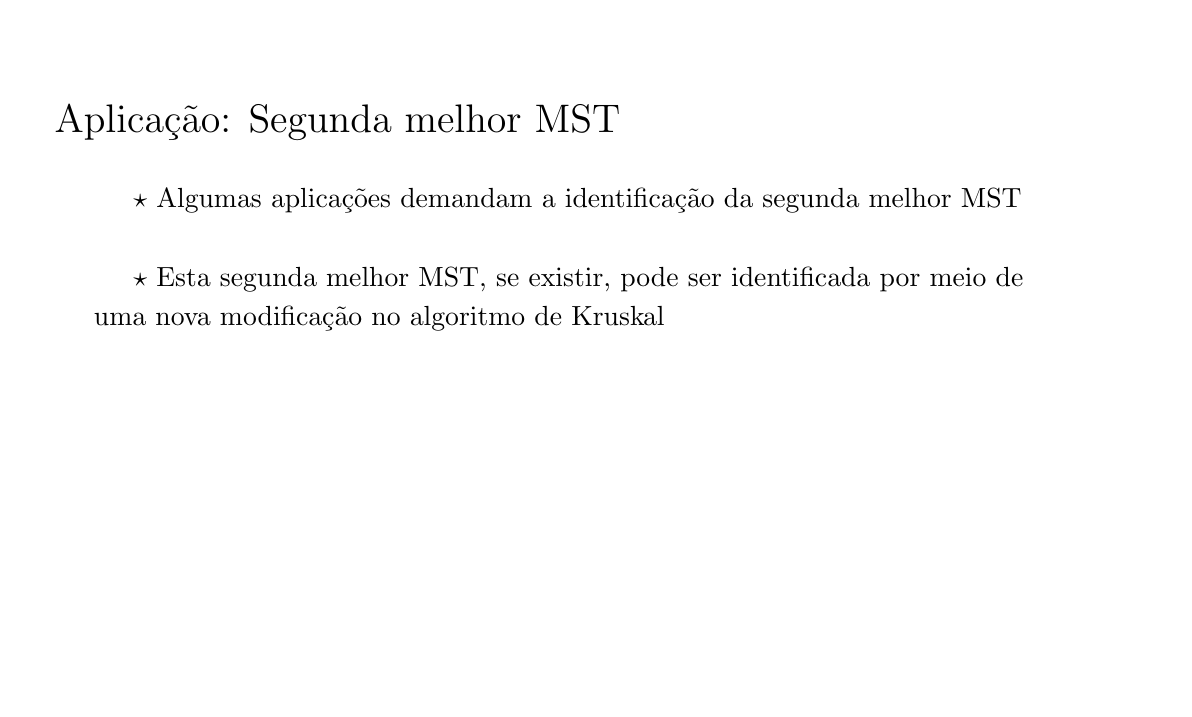
\begin{tikzpicture}
\node[draw,opacity=0] at (0, 0) {x};
\node[draw,opacity=0] at (14, 8) {x};

	\node[anchor=west] (title) at (0.0, 7.0) { \Large \bbbold{Aplicação: Segunda melhor MST} };


	\node[anchor=west] (a) at (1.0, 6.0) { $\star$ \bbtext{Algumas aplicações demandam a identificação da segunda melhor MST} };


	\node[anchor=west] (b) at (1.0, 5.0) { $\star$ \bbtext{Esta segunda melhor MST, se existir, pode ser identificada por meio de } };

	\node[anchor=west] (b1) at (0.5, 4.5) { \bbtext{uma nova modificação no algoritmo de Kruskal} };

\end{tikzpicture}
\end{frame}
\begin{frame}[plain,t]
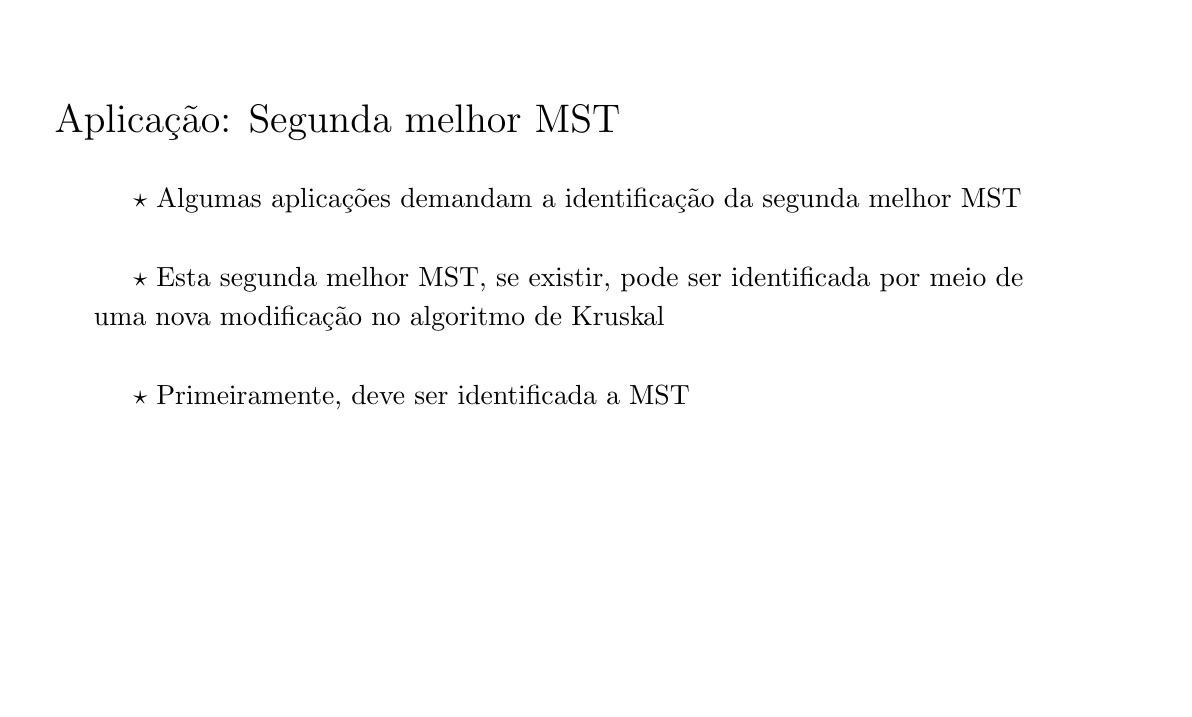
\begin{tikzpicture}
\node[draw,opacity=0] at (0, 0) {x};
\node[draw,opacity=0] at (14, 8) {x};

	\node[anchor=west] (title) at (0.0, 7.0) { \Large \bbbold{Aplicação: Segunda melhor MST} };


	\node[anchor=west] (a) at (1.0, 6.0) { $\star$ \bbtext{Algumas aplicações demandam a identificação da segunda melhor MST} };


	\node[anchor=west] (b) at (1.0, 5.0) { $\star$ \bbtext{Esta segunda melhor MST, se existir, pode ser identificada por meio de } };

	\node[anchor=west] (b1) at (0.5, 4.5) { \bbtext{uma nova modificação no algoritmo de Kruskal} };


	\node[anchor=west] (c) at (1.0, 3.5) { $\star$ \bbtext{Primeiramente, deve ser identificada a MST} };

\end{tikzpicture}
\end{frame}
\begin{frame}[plain,t]
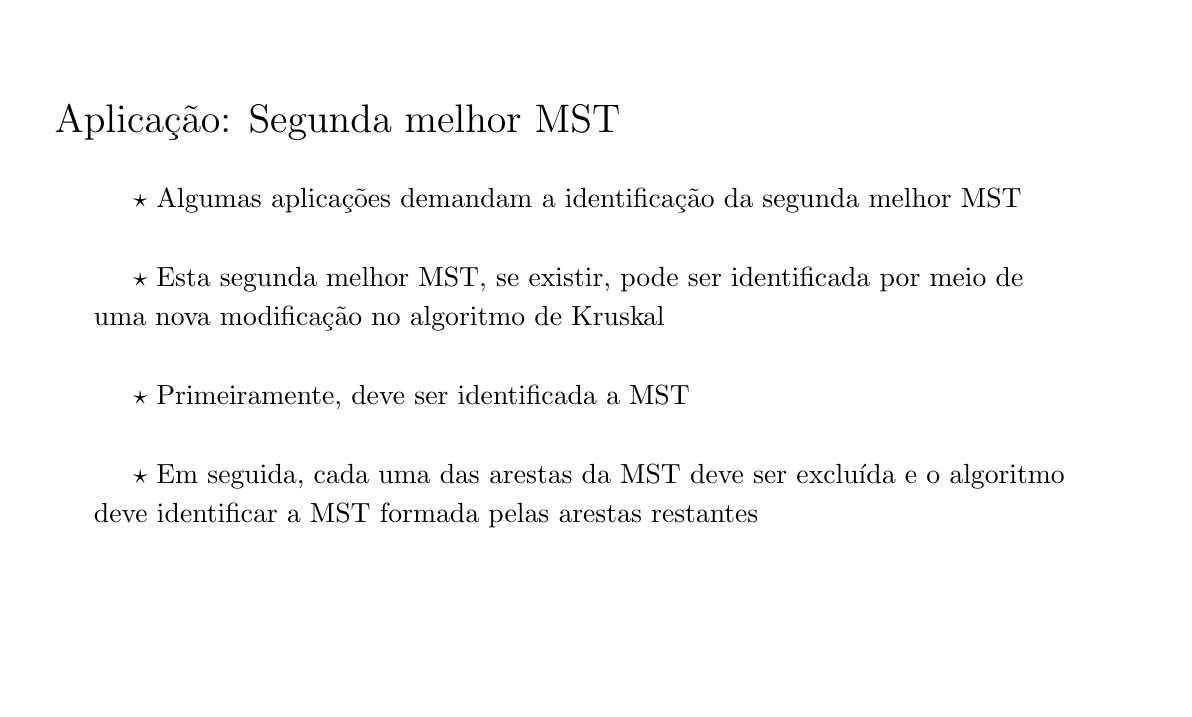
\begin{tikzpicture}
\node[draw,opacity=0] at (0, 0) {x};
\node[draw,opacity=0] at (14, 8) {x};

	\node[anchor=west] (title) at (0.0, 7.0) { \Large \bbbold{Aplicação: Segunda melhor MST} };


	\node[anchor=west] (a) at (1.0, 6.0) { $\star$ \bbtext{Algumas aplicações demandam a identificação da segunda melhor MST} };


	\node[anchor=west] (b) at (1.0, 5.0) { $\star$ \bbtext{Esta segunda melhor MST, se existir, pode ser identificada por meio de } };

	\node[anchor=west] (b1) at (0.5, 4.5) { \bbtext{uma nova modificação no algoritmo de Kruskal} };


	\node[anchor=west] (c) at (1.0, 3.5) { $\star$ \bbtext{Primeiramente, deve ser identificada a MST} };


	\node[anchor=west] (d) at (1.0, 2.5) { $\star$ \bbtext{Em seguida, cada uma das arestas da MST deve ser excluída e o algoritmo} };

	\node[anchor=west] (d1) at (0.5, 2.0) { \bbtext{deve identificar a MST formada pelas arestas restantes} };

\end{tikzpicture}
\end{frame}
\begin{frame}[plain,t]
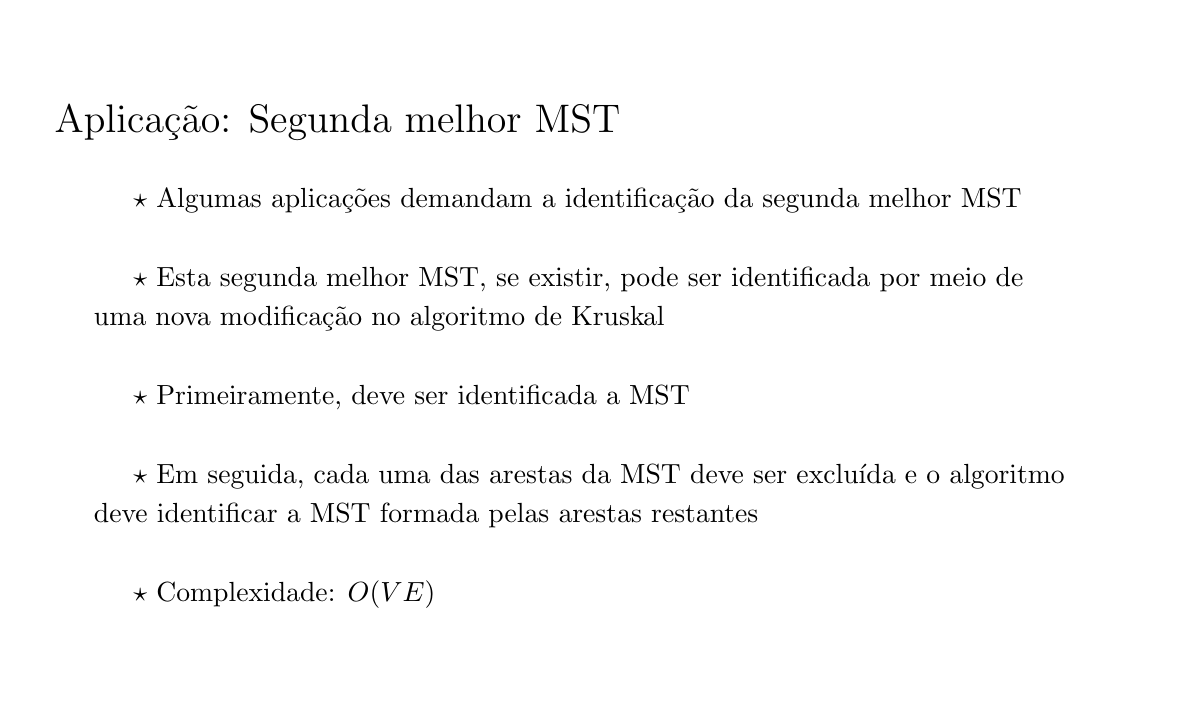
\begin{tikzpicture}
\node[draw,opacity=0] at (0, 0) {x};
\node[draw,opacity=0] at (14, 8) {x};

	\node[anchor=west] (title) at (0.0, 7.0) { \Large \bbbold{Aplicação: Segunda melhor MST} };


	\node[anchor=west] (a) at (1.0, 6.0) { $\star$ \bbtext{Algumas aplicações demandam a identificação da segunda melhor MST} };


	\node[anchor=west] (b) at (1.0, 5.0) { $\star$ \bbtext{Esta segunda melhor MST, se existir, pode ser identificada por meio de } };

	\node[anchor=west] (b1) at (0.5, 4.5) { \bbtext{uma nova modificação no algoritmo de Kruskal} };


	\node[anchor=west] (c) at (1.0, 3.5) { $\star$ \bbtext{Primeiramente, deve ser identificada a MST} };


	\node[anchor=west] (d) at (1.0, 2.5) { $\star$ \bbtext{Em seguida, cada uma das arestas da MST deve ser excluída e o algoritmo} };

	\node[anchor=west] (d1) at (0.5, 2.0) { \bbtext{deve identificar a MST formada pelas arestas restantes} };


	\node[anchor=west] (e) at (1.0, 1.0) { $\star$ \bbbold{Complexidade:} $O(VE)$ };

\end{tikzpicture}
\end{frame}
\begin{frame}[plain,t]
\begin{tikzpicture}
\node[draw,opacity=0] at (0, 0) {x};
\node[draw,opacity=0] at (14, 8) {x};

	\node[draw,very thick,circle] (nodeA) at (6.0, 7.0) { \bbtext{A} };

	\node[draw,very thick,circle] (nodeB) at (10.0, 7.0) { \bbtext{B} };

	\node[draw,very thick,circle] (nodeC) at (12.0, 4.0) { \bbtext{C} };

	\node[draw,very thick,circle] (nodeD) at (8.0, 1.0) { \bbtext{D} };

	\node[draw,very thick,circle] (nodeE) at (4.0, 4.0) { \bbtext{E} };

	\draw[thick](nodeA) to node[above] { \footnotesize \bbinfo{1} } (nodeB);

	\draw[thick](nodeA) to node[above right] { \footnotesize \bbinfo{4} } (nodeC);

	\draw[thick](nodeA) to node[below left,pos=0.2] { \footnotesize \bbinfo{4} } (nodeD);

	\draw[thick](nodeA) to node[left] { \footnotesize \bbinfo{3} } (nodeE);

	\draw[thick](nodeB) to node[above right] { \footnotesize \bbinfo{5} } (nodeC);

	\draw[thick](nodeC) to node[below right] { \footnotesize \bbinfo{5} } (nodeD);

	\draw[thick](nodeC) to node[above, pos=0.3] { \footnotesize \bbinfo{2} } (nodeE);

	\draw[thick](nodeD) to node[below left] { \footnotesize \bbinfo{3} } (nodeE);

\end{tikzpicture}
\end{frame}
\begin{frame}[plain,t]
\begin{tikzpicture}
\node[draw,opacity=0] at (0, 0) {x};
\node[draw,opacity=0] at (14, 8) {x};

	\node[draw,very thick,circle] (nodeA) at (6.0, 7.0) { \bbtext{A} };

	\node[draw,very thick,circle] (nodeB) at (10.0, 7.0) { \bbtext{B} };

	\node[draw,very thick,circle] (nodeC) at (12.0, 4.0) { \bbtext{C} };

	\node[draw,very thick,circle] (nodeD) at (8.0, 1.0) { \bbtext{D} };

	\node[draw,very thick,circle] (nodeE) at (4.0, 4.0) { \bbtext{E} };

	\draw[thick,color=BBCyan,dashed,very thick](nodeA) to node[above] { \footnotesize \bbinfo{1} } (nodeB);

	\draw[thick](nodeA) to node[above right] { \footnotesize \bbinfo{4} } (nodeC);

	\draw[thick](nodeA) to node[below left,pos=0.2] { \footnotesize \bbinfo{4} } (nodeD);

	\draw[thick,color=BBCyan,dashed,very thick](nodeA) to node[left] { \footnotesize \bbinfo{3} } (nodeE);

	\draw[thick](nodeB) to node[above right] { \footnotesize \bbinfo{5} } (nodeC);

	\draw[thick](nodeC) to node[below right] { \footnotesize \bbinfo{5} } (nodeD);

	\draw[thick,color=BBCyan,dashed,very thick](nodeC) to node[above, pos=0.3] { \footnotesize \bbinfo{2} } (nodeE);

	\draw[thick,color=BBCyan,dashed,very thick](nodeD) to node[below left] { \footnotesize \bbinfo{3} } (nodeE);


	\node[anchor=west] (tree) at (0.0, 7.0) { \bbtext{MST} };

	\node[anchor=west] (cost) at (0.0, 6.25) { $c($\bbtext{MST}$) = 9$ };





\end{tikzpicture}
\end{frame}
\begin{frame}[plain,t]
\begin{tikzpicture}
\node[draw,opacity=0] at (0, 0) {x};
\node[draw,opacity=0] at (14, 8) {x};

	\node[draw,very thick,circle] (nodeA) at (6.0, 7.0) { \bbtext{A} };

	\node[draw,very thick,circle] (nodeB) at (10.0, 7.0) { \bbtext{B} };

	\node[draw,very thick,circle] (nodeC) at (12.0, 4.0) { \bbtext{C} };

	\node[draw,very thick,circle] (nodeD) at (8.0, 1.0) { \bbtext{D} };

	\node[draw,very thick,circle] (nodeE) at (4.0, 4.0) { \bbtext{E} };


	\draw[thick](nodeA) to node[above right] { \footnotesize \bbinfo{4} } (nodeC);

	\draw[thick](nodeA) to node[below left,pos=0.2] { \footnotesize \bbinfo{4} } (nodeD);

	\draw[thick,color=BBGreen,dashed,very thick](nodeA) to node[left] { \footnotesize \bbinfo{3} } (nodeE);

	\draw[thick,color=BBGreen,dashed,very thick](nodeB) to node[above right] { \footnotesize \bbinfo{5} } (nodeC);

	\draw[thick](nodeC) to node[below right] { \footnotesize \bbinfo{5} } (nodeD);

	\draw[thick,color=BBGreen,dashed,very thick](nodeC) to node[above, pos=0.3] { \footnotesize \bbinfo{2} } (nodeE);

	\draw[thick,color=BBGreen,dashed,very thick](nodeD) to node[below left] { \footnotesize \bbinfo{3} } (nodeE);


	\node[anchor=west] (tree) at (0.0, 7.0) { \bbtext{Árvore geradora $T_1$} };

	\node[anchor=west] (cost) at (0.0, 6.25) { $c(T_1) = 13$ };










\end{tikzpicture}
\end{frame}
\begin{frame}[plain,t]
\begin{tikzpicture}
\node[draw,opacity=0] at (0, 0) {x};
\node[draw,opacity=0] at (14, 8) {x};

	\node[draw,very thick,circle] (nodeA) at (6.0, 7.0) { \bbtext{A} };

	\node[draw,very thick,circle] (nodeB) at (10.0, 7.0) { \bbtext{B} };

	\node[draw,very thick,circle] (nodeC) at (12.0, 4.0) { \bbtext{C} };

	\node[draw,very thick,circle] (nodeD) at (8.0, 1.0) { \bbtext{D} };

	\node[draw,very thick,circle] (nodeE) at (4.0, 4.0) { \bbtext{E} };

	\draw[thick,color=BBViolet,dashed,very thick](nodeA) to node[above] { \footnotesize \bbinfo{1} } (nodeB);

	\draw[thick,color=BBViolet,dashed,very thick](nodeA) to node[above right] { \footnotesize \bbinfo{4} } (nodeC);

	\draw[thick](nodeA) to node[below left,pos=0.2] { \footnotesize \bbinfo{4} } (nodeD);

	\draw[thick,color=BBViolet,dashed,very thick](nodeA) to node[left] { \footnotesize \bbinfo{3} } (nodeE);


	\draw[thick](nodeC) to node[below right] { \footnotesize \bbinfo{5} } (nodeD);


	\draw[thick,color=BBViolet,dashed,very thick](nodeD) to node[below left] { \footnotesize \bbinfo{3} } (nodeE);


	\node[anchor=west] (tree) at (0.0, 7.0) { \bbtext{Árvore geradora $T_2$} };

	\node[anchor=west] (cost) at (0.0, 6.25) { $c(T_2) = 11$ };













	\draw[thick](nodeB) to node[above right] { \footnotesize \bbinfo{5} } (nodeC);



\end{tikzpicture}
\end{frame}
\begin{frame}[plain,t]
\begin{tikzpicture}
\node[draw,opacity=0] at (0, 0) {x};
\node[draw,opacity=0] at (14, 8) {x};

	\node[draw,very thick,circle] (nodeA) at (6.0, 7.0) { \bbtext{A} };

	\node[draw,very thick,circle] (nodeB) at (10.0, 7.0) { \bbtext{B} };

	\node[draw,very thick,circle] (nodeC) at (12.0, 4.0) { \bbtext{C} };

	\node[draw,very thick,circle] (nodeD) at (8.0, 1.0) { \bbtext{D} };

	\node[draw,very thick,circle] (nodeE) at (4.0, 4.0) { \bbtext{E} };

	\draw[thick,color=BBRed,dashed,very thick](nodeA) to node[above] { \footnotesize \bbinfo{1} } (nodeB);

	\draw[thick,color=BBRed,dashed,very thick](nodeA) to node[above right] { \footnotesize \bbinfo{4} } (nodeC);

	\draw[thick](nodeA) to node[below left,pos=0.2] { \footnotesize \bbinfo{4} } (nodeD);



	\draw[thick](nodeC) to node[below right] { \footnotesize \bbinfo{5} } (nodeD);

	\draw[thick,color=BBRed,dashed,very thick](nodeC) to node[above, pos=0.3] { \footnotesize \bbinfo{2} } (nodeE);

	\draw[thick,color=BBRed,dashed,very thick](nodeD) to node[below left] { \footnotesize \bbinfo{3} } (nodeE);


	\node[anchor=west] (tree) at (0.0, 7.0) { \bbtext{Árvore geradora $T_3$} };

	\node[anchor=west] (cost) at (0.0, 6.25) { $c(T_3) = 10$ };













	\draw[thick](nodeB) to node[above right] { \footnotesize \bbinfo{5} } (nodeC);







\end{tikzpicture}
\end{frame}
\begin{frame}[plain,t]
\begin{tikzpicture}
\node[draw,opacity=0] at (0, 0) {x};
\node[draw,opacity=0] at (14, 8) {x};

	\node[draw,very thick,circle] (nodeA) at (6.0, 7.0) { \bbtext{A} };

	\node[draw,very thick,circle] (nodeB) at (10.0, 7.0) { \bbtext{B} };

	\node[draw,very thick,circle] (nodeC) at (12.0, 4.0) { \bbtext{C} };

	\node[draw,very thick,circle] (nodeD) at (8.0, 1.0) { \bbtext{D} };

	\node[draw,very thick,circle] (nodeE) at (4.0, 4.0) { \bbtext{E} };

	\draw[thick,color=BBGray,dashed,very thick](nodeA) to node[above] { \footnotesize \bbinfo{1} } (nodeB);


	\draw[thick,color=BBGray,dashed,very thick](nodeA) to node[below left,pos=0.2] { \footnotesize \bbinfo{4} } (nodeD);

	\draw[thick,color=BBGray,dashed,very thick](nodeA) to node[left] { \footnotesize \bbinfo{3} } (nodeE);


	\draw[thick](nodeC) to node[below right] { \footnotesize \bbinfo{5} } (nodeD);

	\draw[thick,color=BBGray,dashed,very thick](nodeC) to node[above, pos=0.3] { \footnotesize \bbinfo{2} } (nodeE);



	\node[anchor=west] (tree) at (0.0, 7.0) { \bbtext{Árvore geradora $T_4$} };

	\node[anchor=west] (cost) at (0.0, 6.25) { $c(T_4) = 10$ };













	\draw[thick](nodeB) to node[above right] { \footnotesize \bbinfo{5} } (nodeC);













	\draw[thick](nodeA) to node[above right] { \footnotesize \bbinfo{4} } (nodeC);

\end{tikzpicture}
\end{frame}
\begin{frame}[plain,t]

\inputsnippet{cpp}{48}{67}{codes/second_best.cpp}

\end{frame}
\begin{frame}[plain,t]

\inputsnippet{cpp}{69}{83}{codes/second_best.cpp}

\end{frame}
\begin{frame}[plain,t]
\begin{tikzpicture}
\node[draw,opacity=0] at (0, 0) {x};
\node[draw,opacity=0] at (14, 8) {x};

	\node[anchor=west] (title) at (0.0, 6.0) { \Large \bbbold{Problemas sugeridos} };

	\node[anchor=west] (a) at (1.0, 5.0) { $1.$ \bbtext{Codechef CHEFELEC -- Chefland and Electricity} };

	\node[anchor=west] (b) at (1.0, 4.0) { $2.$ \bbtext{OJ 10369 -- Artic Network} };

	\node[anchor=west] (c) at (1.0, 3.0) { $3.$ \bbtext{OJ 10600 -- ACM Contest and Blackout} };

	\node[anchor=west] (d) at (1.0, 2.0) { $4.$ \bbtext{SPOJ EC\_MODE -- Modems} };

\end{tikzpicture}
\end{frame}
\begin{frame}[plain,t]
\begin{tikzpicture}
\node[draw,opacity=0] at (0, 0) {x};
\node[draw,opacity=0] at (14, 8) {x};

	\node[anchor=west] (title) at (0.0, 7.0) { \Large \bbbold{Referências} };

	\node[anchor=west] (a) at (1.0, 6.0) { $1.$ \bbtext{\bbbold{CP-Algorithm}. \bbenglish{Minimum spanning tree -- Kruskal's algorithm}, acesso em} };

	\node[anchor=west] (a1) at (2.0, 5.5) { \bbtext{24/08/2021.} };

	\node[anchor=west] (b) at (1.0, 4.5) { $2.$ \bbbold{HALIM}, \bbtext{Felix}; \bbbold{HALIM}, \bbtext{Steve}. \bbenglish{Competitive Programming 3,} \bbtext{2010.} };

	\node[anchor=west] (c) at (1.0, 3.5) { $3.$ \bbbold{LAAKSONEN}, \bbtext{Antti}. \bbenglish{Competitive Programmer's Handbook,} \bbtext{2018.} };

	\node[anchor=west] (d) at (1.0, 2.5) { $4.$ \bbbold{Wikipédia}. \bbenglish{Joseph Kruskal,} \bbtext{acesso em 24/08/2021.} };

	\node[anchor=west] (e) at (1.0, 1.5) { $5.$ \bbbold{Wikipédia}. \bbenglish{Kruskal's algorithm,} \bbtext{acesso em 24/08/2021.} };

\end{tikzpicture}
\end{frame}
\end{document}
